cuts.tex

% Data Analysis

The azimuthal distribution of these high quality tracks is not fully uniform due to inefficient regions in the SPD.
This is compensated by tracks \textit{without} reconstructed track points in the SPD. 
For those tracks, the primary vertex is used as an additional constraint in the track fitting to improve the momentum resolution. 
This approach yields a very uniform tracking efficiency within the acceptance, which is needed to avoid geometrical biases of the jet reconstruction algorithm caused by a non-uniform density of reconstructed  tracks.
For the analyzed data, the additional tracks (without SPD track points) constitute approximately 4.3\% of the used track sample. 

For tracks with reconstructed track points close to the vertex (measured by the SPD), a momentum resolution of  0.8\% (3.8\%) for $\pt = 1$~GeV/$c$ (50 GeV/$c$) is reached \cite{Abelev:2014ffa}. 

To estimate and subtract the background contribution to the jet energy we employ the method described in \cite{Adam:2015hoa,Abelev:2013kqa}. 

In $\pPb$ collisions, however, the multiplicity density is two orders of magnitude smaller than in central $\PbPb$ collisions \cite{ALICE:2012xs} and a corresponding reduction of the jet background is expected. 
In this analysis, an improved estimate for the more sparse environment of $\pPb$ events a variation \cite{Adam:2015hoa} of the approach described in \cite{Chatrchyan:2012tt} was employed. 

Note, that in this analysis jets are used as a tag of the hard scatterings and we are not interested in their \pt\ spectrum (reported in )
Consequently, the hard scatterings are tagged with anti-\kt\ jets with $\ptjet > 10 \gevc$ and $20 \gevc$ that is corrected on an event-by-event basis for the event background $\rho \Ajet$, such that $\ptjet = \pt^{{\rm raw~anti-\kt}} - \rho \Ajet$.

The jet area \Ajet\ is determined with the so-called \emph{active area} algorithm \cite{Cacciari:2008gn} with \emph{ghost particles} of 0.005 area (rad). 

a variation  of the approach described in \cite{Chatrchyan:2012tt} was employed. 


%%% results

The normalized spectra of OC $\Vzeros$ are shown in
figure~\ref{fig:c05RestulsCompOCPtJ10} and
figure~\ref{fig:c05RestulsCompOCPtJ20} with $\pT^{\rm jet}>10~\GeVc$ and
$\pT^{\rm jet}>20~\GeVc$, respectively.
The charged jets are reconstructed with $R_{\rm jet}=0.4$.
In general, the difference between the OC $\Vzeros$ with
different $\Delta R_{\rm cut}$ is small ($\sim 2\%$).
With smaller $\Delta R_{\rm cut}$ (e.g. $\Delta R_{\rm cut}=0.4$),
the correlations between the OC component and JC $\Vzeros$ is stronger.
And its normalized spectrum is systematically higher
than the ones with  larger $\Delta R_{\rm cut}$.


The normalized $\pT$ spectra for different type of $\Vzeros$ are
compared in figure~\ref{fig:c05RestulsCompJCPtJ10} and
figure~\ref{fig:c05RestulsCompJCPtJ20}
with $\pT^{\rm jet}>10~\GeVc$ and $\pT^{\rm jet}>20~\GeVc$, respectively.
As expected, the spectra of OC and NJ $\Vzeros$ are very close to the that
of the inclusive $\Vzeros$ in the low $\pT$ region since the
inclusive $\Vzero$ production is dominated by the $\Vzeros$ from
the underlying events.
In the high $\pT$ region,
the spectra of OC $\Vzeros$ is harder than that of the inclusive $\Vzeros$
and the spectra of NJ $\Vzeros$ is softer than the inclusive ones.
As mentioned in section~\ref{sec:c05EstiV0sUE} the OC $\Vzeros$ may include
the component come from the jets excluded by the jet selection.
And the contribution from the $\Vzeros$ produced inside the jets are
highly suppressed in the sample of the NJ $\Vzeros$ and it makes its
spectrum is softer than that of the inclusive $\Vzeros$.
Despite this difference, the spectra of both the OC and NJ $\Vzeros$
are much softer than that of the JC $\Vzeros$ (as expected,
the high $\pT$ $\Vzero$ are mainly contributed by the jet production),
the uncertainty introduced by the UE $\Vzero$ subtraction should be
small in the high $\pT$ region.



%%% UE

\section{$\Vzero$ yields in the underlying event}
\label{sec:c05EstiV0sUE}

To obtain the spectra of $\Vzeros$ produced in the jets,
the $\Vzeros$ produced in the underlying events ({\bf UE $\mathbf\Vzeros$})
have to be subtracted from the yield of JC $\Vzeros$.
The basic idea is to use the $\Vzeros$ outside the jet cone to estimate
the density of the UE $\Vzeros$ inside jet cone.
But there are two effects which bias the underlying $\Vzero$ evaluation:
\begin{itemize}
\item the $\Vzeros$ outside the selected jets could be
      matched with the excluded jets which are rejected by
      the $\pT$ and $\eta$ cuts of the jet selection;
\item due to the detector response and the jet reconstruction efficiency,
      the physical jets associated to the $\Vzeros$ could be lost by the
      jet finder.
\end{itemize}

In this case, we use two different methods to estimate underlying $\Vzeros$:
\begin{itemize}
\item $\Vzeros$ outside jet cone ({\bf OC $\mathbf\Vzeros$}):
      \begin{equation}\label{eq:c05OCV0s}
      \Delta R_{\Vzero-{\rm jet}}>R_{\rm cut},
      \end{equation}
      where, $R_{\rm cut}$ is a given threshold of the distance between the
      $\Vzero$ and jet axis in $\eta-\phi$ plane;
\item $\Vzeros$ in events without any selected jet ({\bf NJ $\mathbf\Vzeros$}).
\end{itemize}

According to the definitoin,
the OC $\Vzeros$ are selected in the same event sample as the JC $\Vzeros$
and they can include both the $\Vzeros$ in the excluded jets and
the physical jets lost by the jet finder,
they have a strong correlation to the $\Vzeros$ produced in the jets.
On the other hand, if the $\pT$ threshold used to select the jet is low enough,
we do not expect there would be a strong hard scattering in the NJ events,
and the probability for the NJ $\Vzeros$ to match to the physical jets
is lower and their correlations to the $\Vzeros$ produced in the jets
is weaker.

In this analysis,
the JC $\Vzeros$ and the OC $\Vzeros$ are selected in the two open
jet $\pT$ bins: $\pT^{\rm jet}>10~\GeVc$ and $\pT^{\rm jet}>20~\GeVc$.
The {\bf corrected} jet $\pT$ in eq.~(\ref{eq:c04DefEstiJetPT}) is used
for the jet selection.
The NJ $\Vzeros$ are defined in the event without jet
in {\bf measured} $\pT>5~\GeVc$.
The uncertainly on UE $\Vzero$ estimation is given by the
difference between the OC and NJ $\Vzeros$.

%% V0 reconstruction

\begin{figure}[htb]
\begin{center}
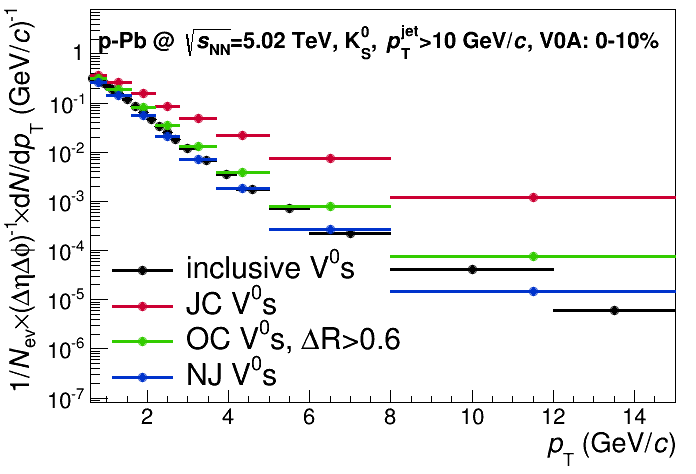
\includegraphics[width=.32\textwidth]{c05Results/cKshort_Comp_JC_JE_V0A_000_010_PtJ10}
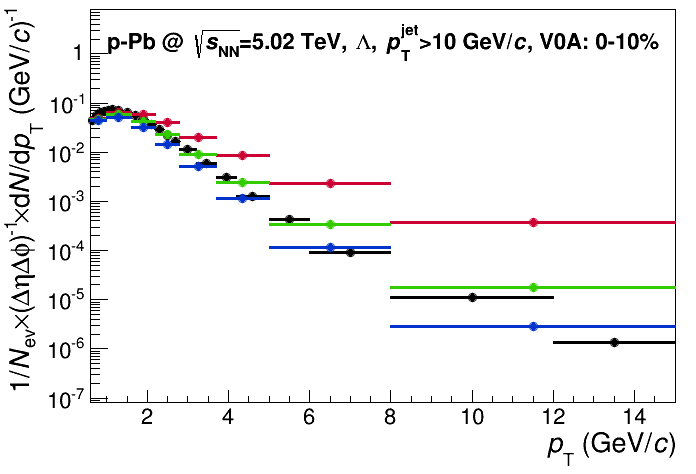
\includegraphics[width=.32\textwidth]{c05Results/cLambda_Comp_JC_JE_V0A_000_010_PtJ10}
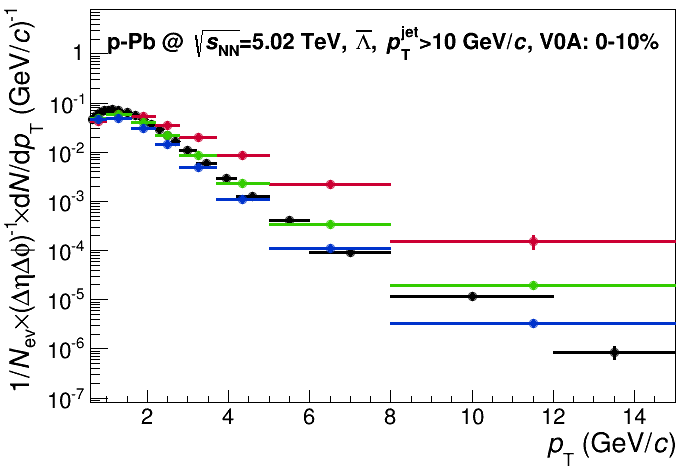
\includegraphics[width=.32\textwidth]{c05Results/cAntiLa_Comp_JC_JE_V0A_000_010_PtJ10}
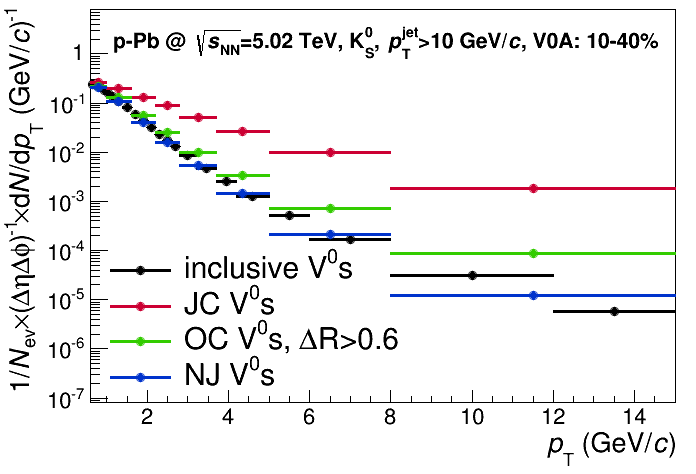
\includegraphics[width=.32\textwidth]{c05Results/cKshort_Comp_JC_JE_V0A_010_040_PtJ10}
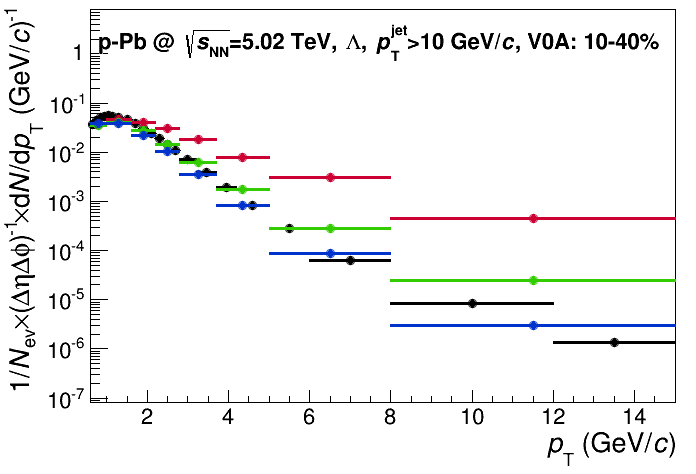
\includegraphics[width=.32\textwidth]{c05Results/cLambda_Comp_JC_JE_V0A_010_040_PtJ10}
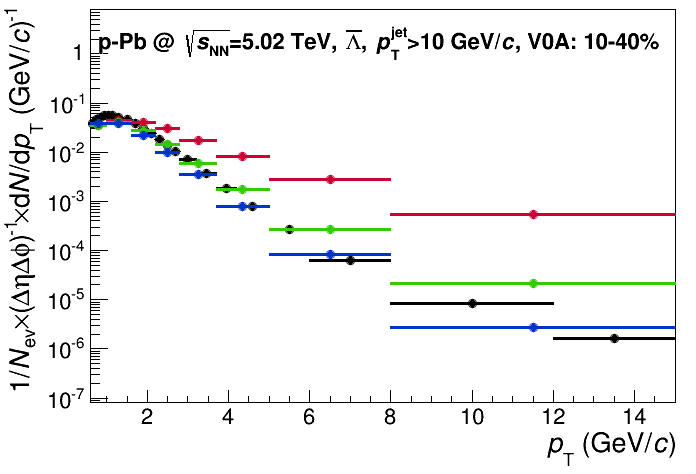
\includegraphics[width=.32\textwidth]{c05Results/cAntiLa_Comp_JC_JE_V0A_010_040_PtJ10}
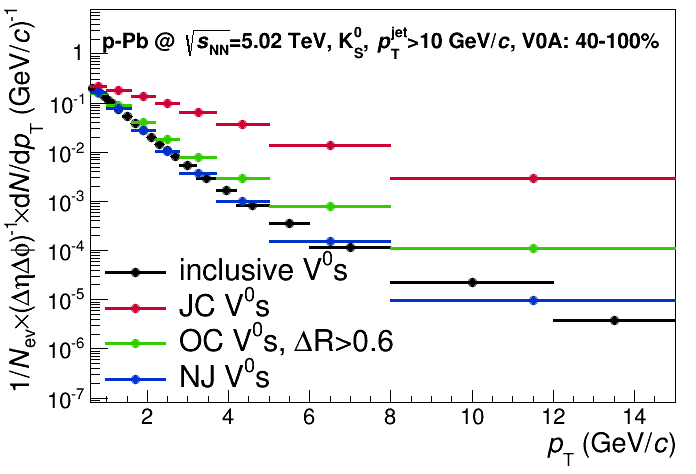
\includegraphics[width=.32\textwidth]{c05Results/cKshort_Comp_JC_JE_V0A_040_100_PtJ10}
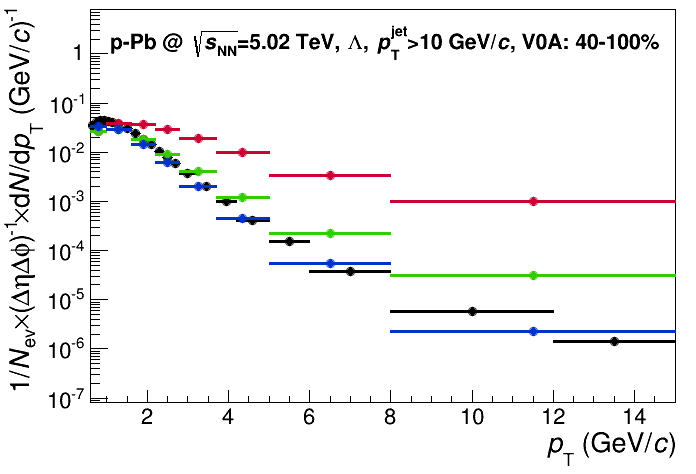
\includegraphics[width=.32\textwidth]{c05Results/cLambda_Comp_JC_JE_V0A_040_100_PtJ10}
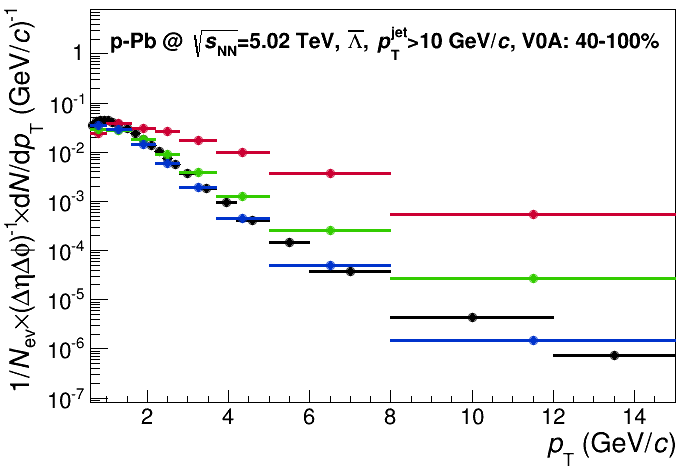
\includegraphics[width=.32\textwidth]{c05Results/cAntiLa_Comp_JC_JE_V0A_040_100_PtJ10}
\caption{Normalized JC $\Vzeros$ and UE $\Vzeros$ in $\pT^{\rm jet}>10~\GeVc$,
         results are compared to the inclusive $\Vzeros$.}
\label{fig:c05RestulsCompJCPtJ10}
\end{center}
\end{figure}

\begin{figure}[htb]
\begin{center}
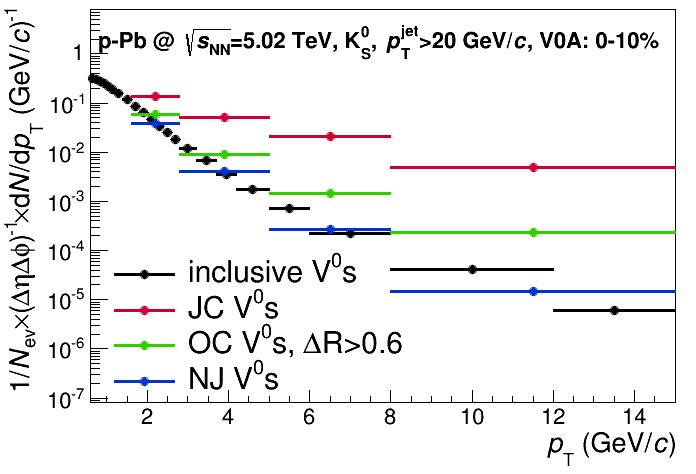
\includegraphics[width=.32\textwidth]{c05Results/cKshort_Comp_JC_JE_V0A_000_010_PtJ20}
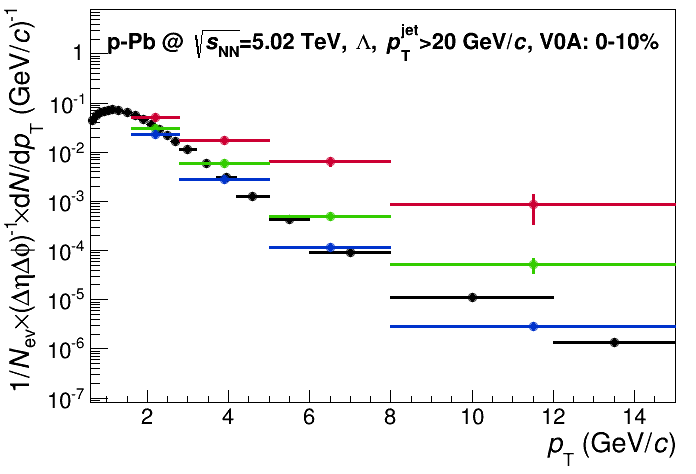
\includegraphics[width=.32\textwidth]{c05Results/cLambda_Comp_JC_JE_V0A_000_010_PtJ20}
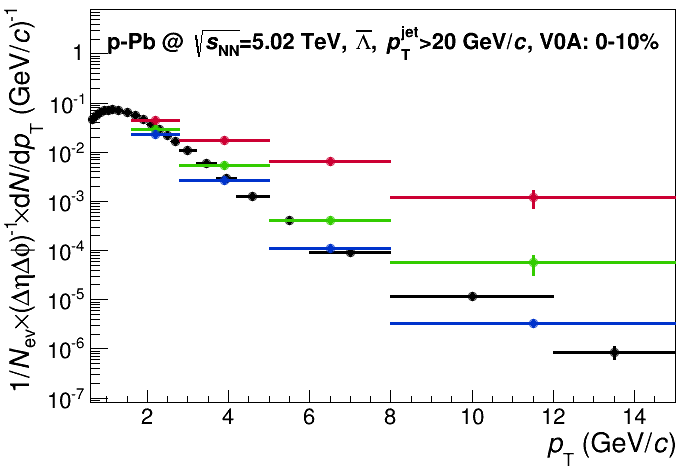
\includegraphics[width=.32\textwidth]{c05Results/cAntiLa_Comp_JC_JE_V0A_000_010_PtJ20}
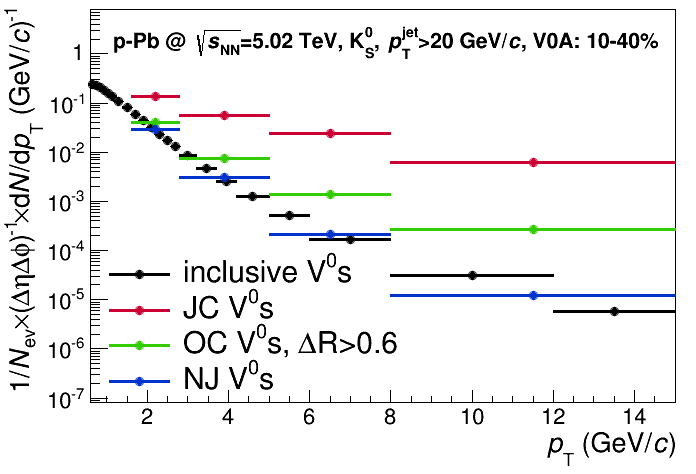
\includegraphics[width=.32\textwidth]{c05Results/cKshort_Comp_JC_JE_V0A_010_040_PtJ20}
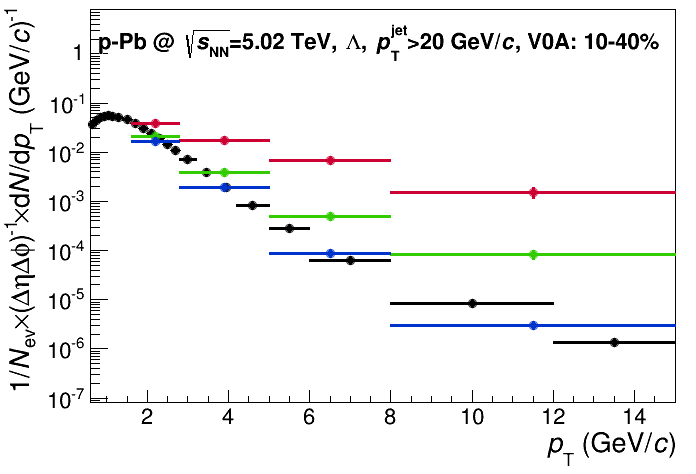
\includegraphics[width=.32\textwidth]{c05Results/cLambda_Comp_JC_JE_V0A_010_040_PtJ20}
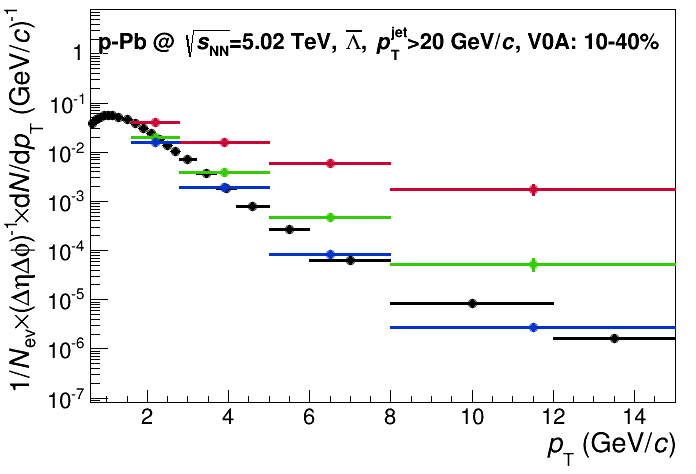
\includegraphics[width=.32\textwidth]{c05Results/cAntiLa_Comp_JC_JE_V0A_010_040_PtJ20}
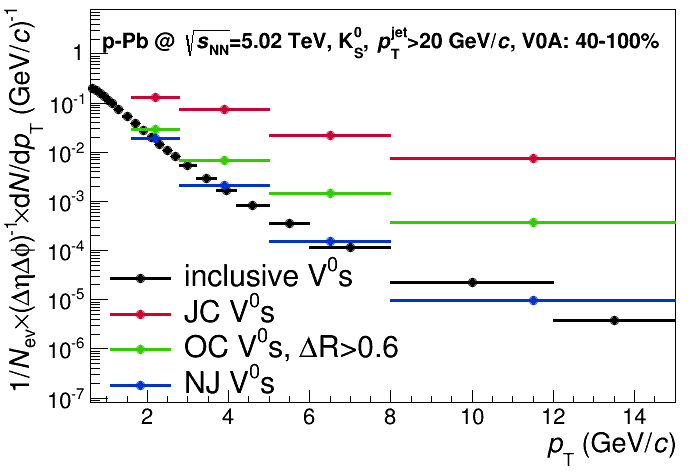
\includegraphics[width=.32\textwidth]{c05Results/cKshort_Comp_JC_JE_V0A_040_100_PtJ20}
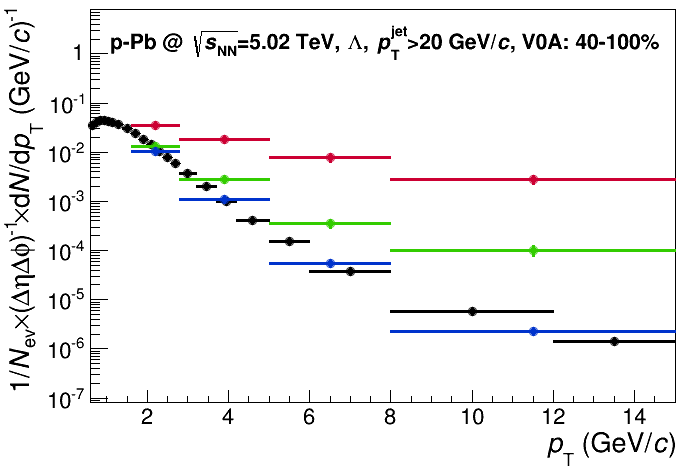
\includegraphics[width=.32\textwidth]{c05Results/cLambda_Comp_JC_JE_V0A_040_100_PtJ20}
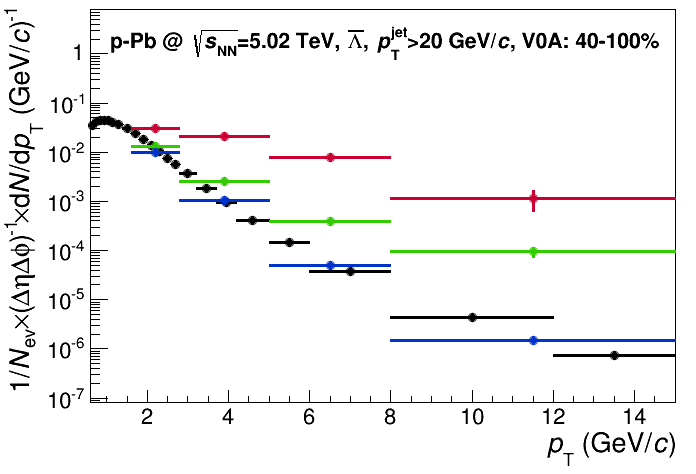
\includegraphics[width=.32\textwidth]{c05Results/cAntiLa_Comp_JC_JE_V0A_040_100_PtJ20}
\caption{Normalized JC $\Vzeros$ and UE $\Vzeros$ in $\pT^{\rm jet}>20~\GeVc$,
         results are compared to the inclusive $\Vzeros$.}
\label{fig:c05RestulsCompJCPtJ20}
\end{center}
\end{figure}



\subsection{Underlying background subtraction}\label{sec:c05NormV0s}

The corrected spectrum of any type of $\Vzeros$
is given by:
\begin{equation}\label{eq:c05EffiCorrV0s}
\frac{{\rm d}N}{{\rm d}\pT}=m(\pT)/\varepsilon_{\rm RD}(\pT),
\end{equation}
where $m(\pT)$ is number of $\Vzeros$ in the given $\pT$ bin after the
bin counting subtraction,
$\varepsilon_{\rm RD}(\pT)$ is the corrected $\Vzero$ efficiency by the
scaling procedure in eq.~(\ref{eq:c05CorrEffImp}).

Since the UE $\Vzeros$ are used to estimate the UE background per acceptance
area density inside the jet cone,
to obtain the $\Vzeros$ produced in jets ({\bf JE $\mathbf\Vzeros$}),
we normalize the yields of both JC and UE $\Vzeros$ to the
per-event acceptance area unit to subtract the UE $\Vzero$ background:
\begin{equation}\label{eq:c05NormV0sJE}
\frac{{\rm d}M_{\rm JE}}{{\rm d}\pT}=
\frac{{\rm d}M_{\rm JC}}{{\rm d}\pT}-\frac{{\rm d}M_{\rm UE}}{{\rm d}\pT},
\end{equation}
where, for the JC and UE $\Vzeros$ the term ${\rm d}M/{\rm d}\pT$ is given by:
\begin{equation}\label{eq:c05NormCorrV0s}
\frac{{\rm d}M_{\rm JC/UE}}{{\rm d}\pT}=
\frac{1}{N_{\rm JC/UE}^{\rm ev}}\times\frac{1}{\Delta\eta\Delta\phi}\times
\frac{{\rm d}N_{\rm JC/UE}}{{\rm d}\pT}.
\end{equation}
In eq.~(\ref{eq:c05NormCorrV0s}),
the term ${\rm d}N_{\rm JC/UE}/{\rm d}\pT$ is the corrected JC or
UE $\Vzero$ spectrum defined in eq.~(\ref{eq:c05EffiCorrV0s}),
$N_{\rm JC/UE}^{\rm ev}$ is the corresponding number of JC or UE events and
$\Delta\eta\times\Delta\phi$ is the per-event acceptance area for
the JC or UE $\Vzeros$.

For the JC or OC $\Vzeros$, since they are obtained in the events have at
least one selected jet in $\pT^{\rm jet}>\pT^{\min}$~\footnote{As discussed
in section~\ref{sec:c05EstiV0sUE},
there are two set of values are chosen
for the $\pT^{\min}$: $\pT^{\min}=10~\GeVc$ and $\pT^{\min}=20~\GeVc$ in
this analysis.},
the $N_{\rm JC/OC}^{\rm ev}$ for the JC or OC $\Vzeros$ is number of events
with at least one selected jet in  $\pT^{\rm jet}>\pT^{\min}$.
For NJ $\Vzeros$, the $N_{\rm NJ}^{\rm ev}$ is the number of events have
no jet in $\pT>5~\GeVc$.

According to the definition,
the per-event acceptance area for NJ $\Vzeros$ is equal to the
acceptance of the inclusive $\Vzero$ define in section~\ref{sec:c05DefAcc}:
\begin{equation}
[\Delta\eta\times\Delta\phi]_{\rm NJ}=2\times 0.75\times 2\pi.
\end{equation}

Concerning the calculation of the per-event acceptance area for the JC or
OC $\Vzeros$ ($[\Delta\eta\times\Delta\phi]_{\rm JC/OC}$),
the following MC approach is adopted:
\begin{enumerate}
\item generate the a given number of testing particles with the
      randomized $\eta$ and $\phi$ in the $\Vzero$ acceptance according to the
      $\eta-\phi$ distribution of the the JC or OC $\Vzero$ candidates (in this
      analysis, $10^{3}$ testing particles are generated in each event),
\item match the testing particles to the jets in each given event
      and count the numbers of the testing particles inside and outside
      the jet cones;
\item the ratio of the number of the JC/OC particles and the number of
      total generated particles gives the fraction of acceptance for
      the JC/OC $\Vzeros$ in the given event;
\item the final acceptance correction factor of JC/OC $\Vzeros$ is given
      by the average of the event-by-event acceptance fraction.
\end{enumerate}

\begin{figure}[htb]
\begin{center}
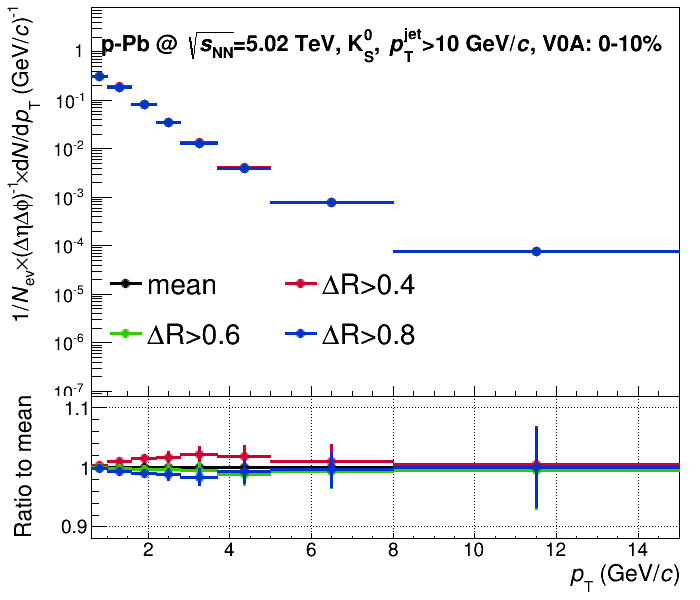
\includegraphics[width=.32\textwidth]{c05Results/cKshort_Comp_OC_JE_V0A_000_010_PtJ10}
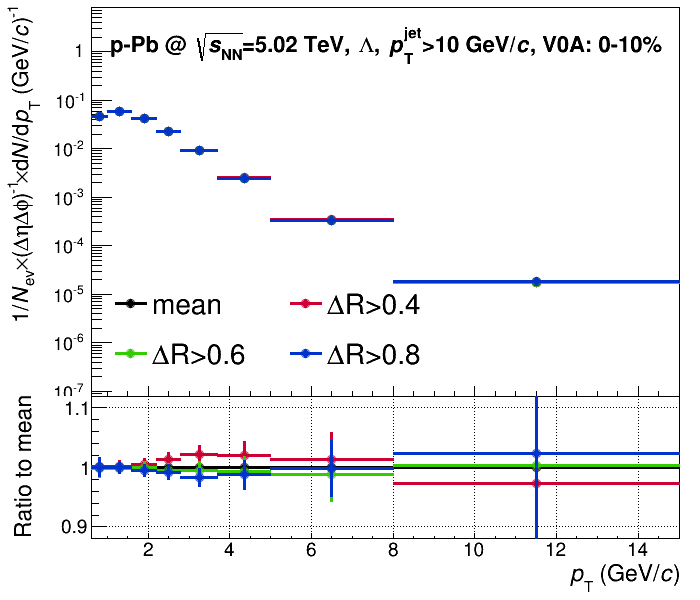
\includegraphics[width=.32\textwidth]{c05Results/cLambda_Comp_OC_JE_V0A_000_010_PtJ10}
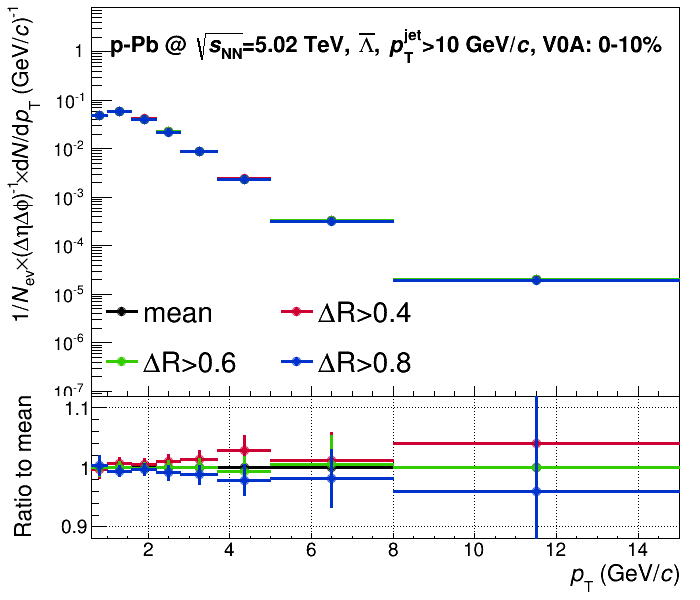
\includegraphics[width=.32\textwidth]{c05Results/cAntiLa_Comp_OC_JE_V0A_000_010_PtJ10}
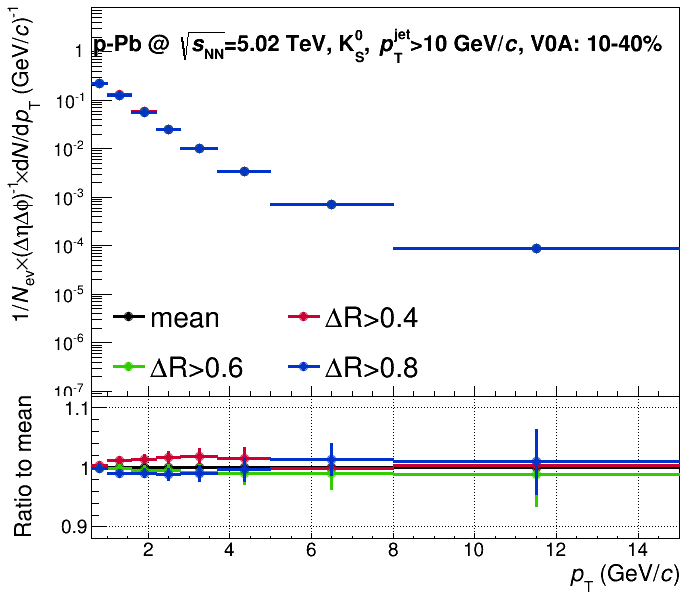
\includegraphics[width=.32\textwidth]{c05Results/cKshort_Comp_OC_JE_V0A_010_040_PtJ10}
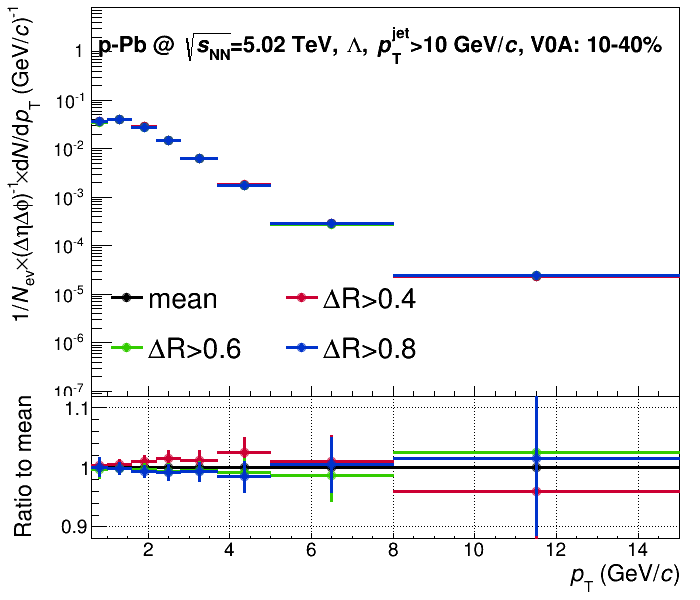
\includegraphics[width=.32\textwidth]{c05Results/cLambda_Comp_OC_JE_V0A_010_040_PtJ10}
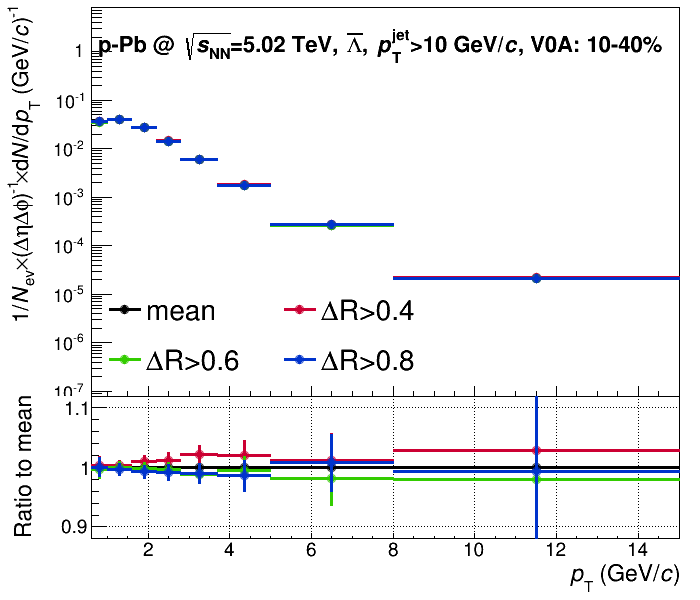
\includegraphics[width=.32\textwidth]{c05Results/cAntiLa_Comp_OC_JE_V0A_010_040_PtJ10}
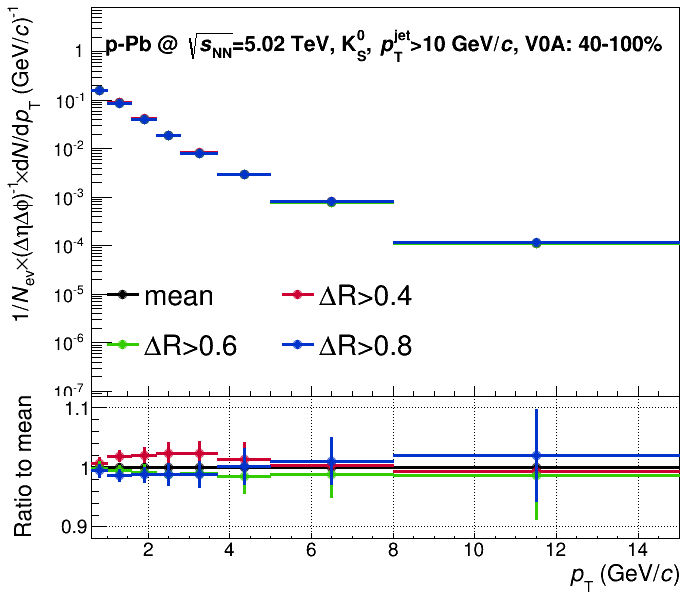
\includegraphics[width=.32\textwidth]{c05Results/cKshort_Comp_OC_JE_V0A_040_100_PtJ10}
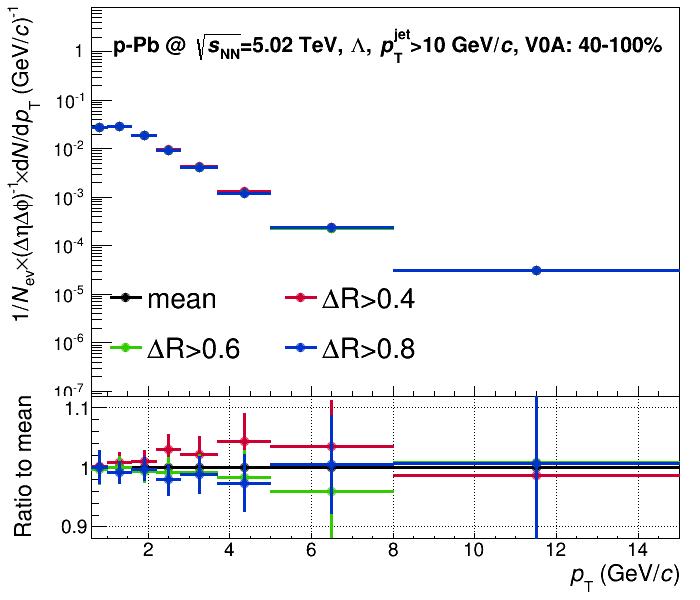
\includegraphics[width=.32\textwidth]{c05Results/cLambda_Comp_OC_JE_V0A_040_100_PtJ10}
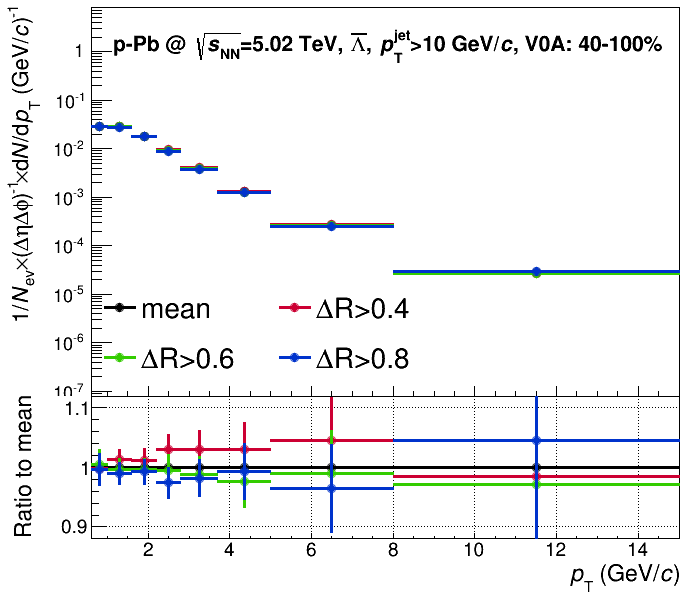
\includegraphics[width=.32\textwidth]{c05Results/cAntiLa_Comp_OC_JE_V0A_040_100_PtJ10}
\caption{Normalized ${\rm OC}~\Vzeros$ with different $\Delta R$ in
         $\pT^{\rm jet}>10~\GeVc$.}
\label{fig:c05RestulsCompOCPtJ10}
\end{center}
\end{figure}

\begin{figure}[htb]
\begin{center}
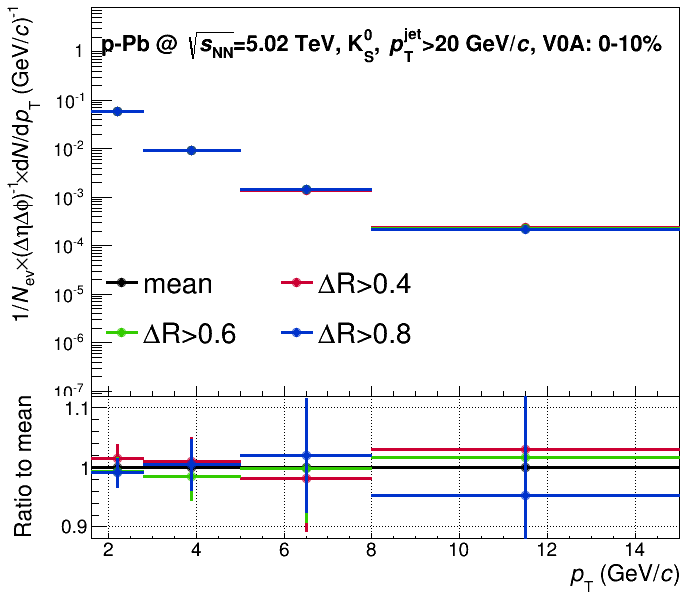
\includegraphics[width=.32\textwidth]{c05Results/cKshort_Comp_OC_JE_V0A_000_010_PtJ20}
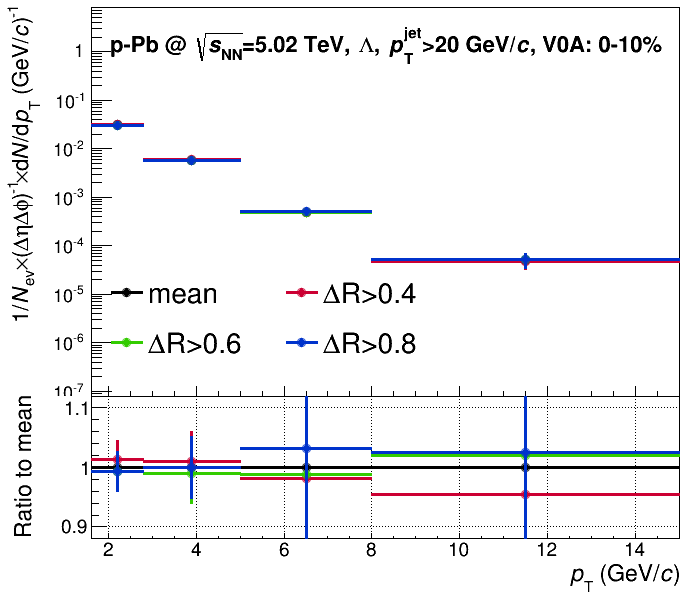
\includegraphics[width=.32\textwidth]{c05Results/cLambda_Comp_OC_JE_V0A_000_010_PtJ20}
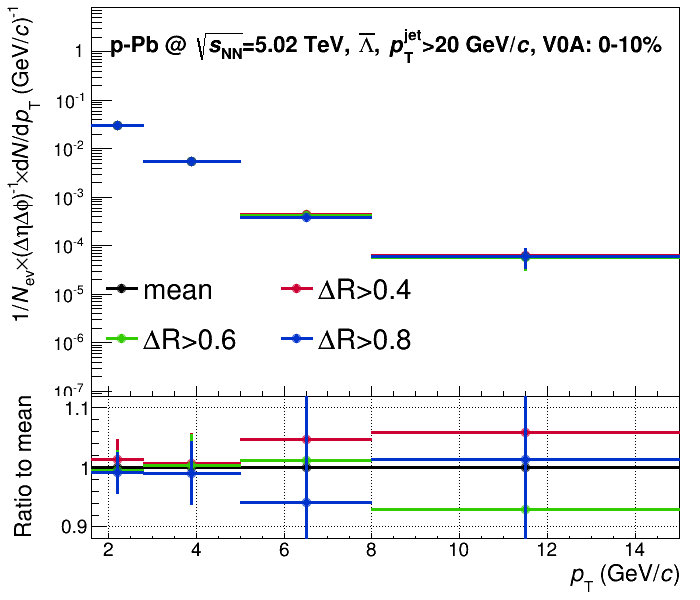
\includegraphics[width=.32\textwidth]{c05Results/cAntiLa_Comp_OC_JE_V0A_000_010_PtJ20}
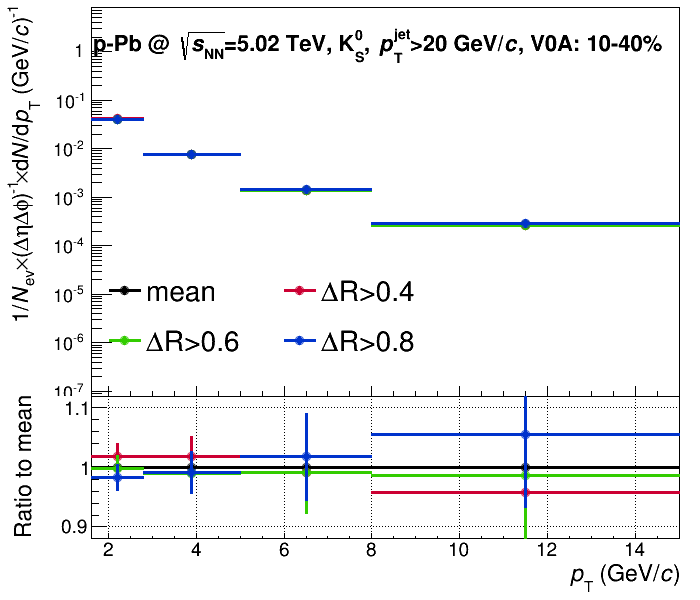
\includegraphics[width=.32\textwidth]{c05Results/cKshort_Comp_OC_JE_V0A_010_040_PtJ20}
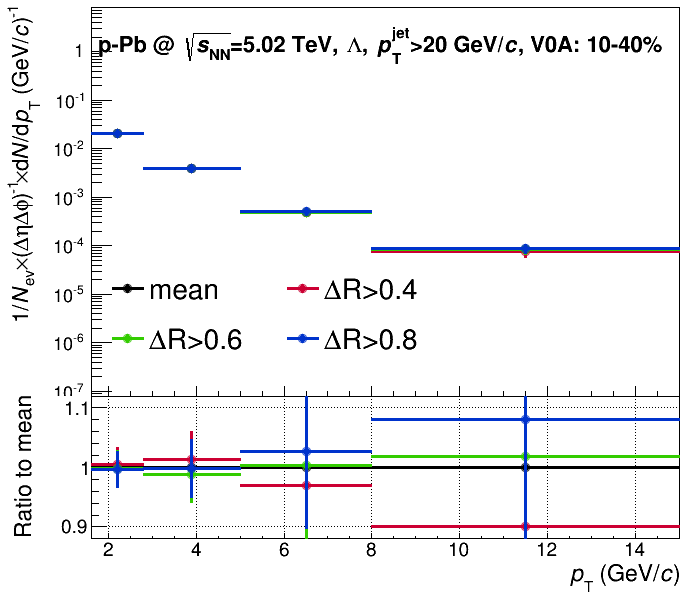
\includegraphics[width=.32\textwidth]{c05Results/cLambda_Comp_OC_JE_V0A_010_040_PtJ20}
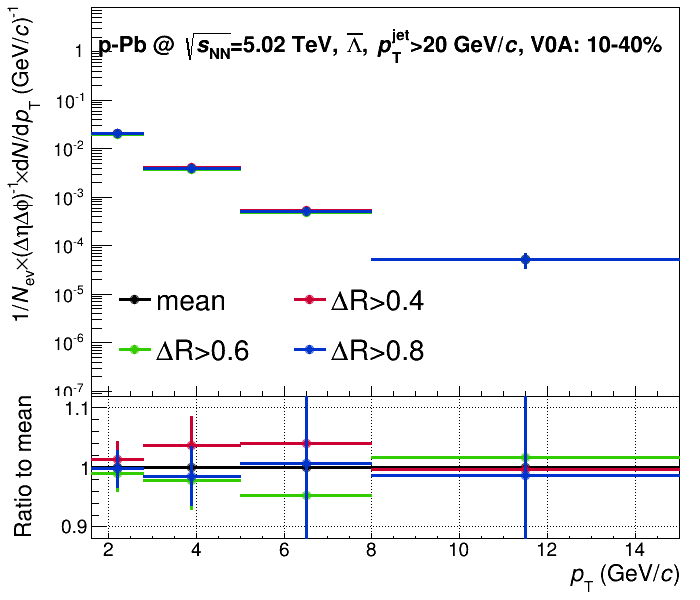
\includegraphics[width=.32\textwidth]{c05Results/cAntiLa_Comp_OC_JE_V0A_010_040_PtJ20}
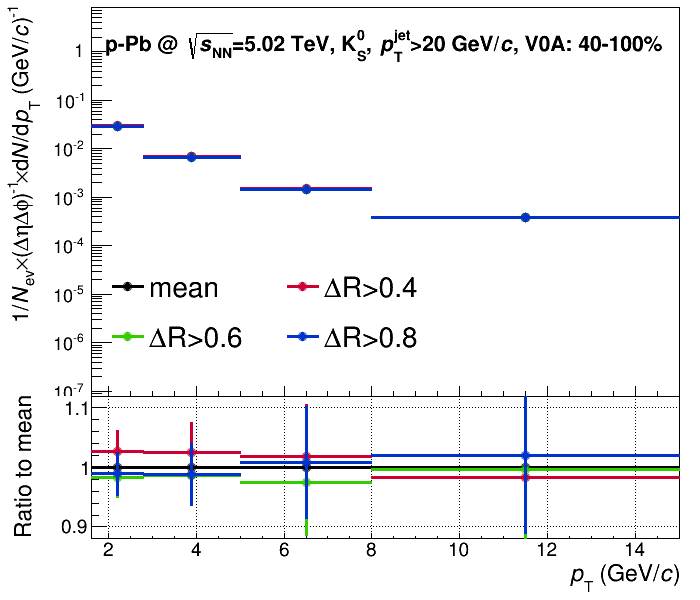
\includegraphics[width=.32\textwidth]{c05Results/cKshort_Comp_OC_JE_V0A_040_100_PtJ20}
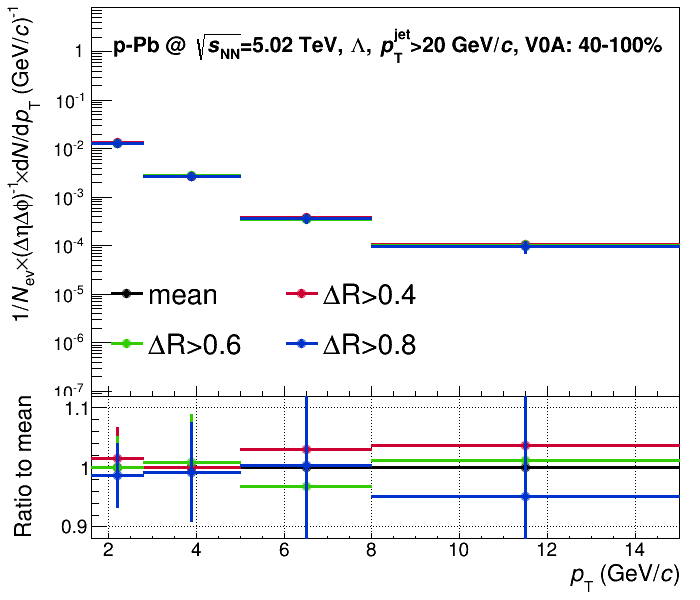
\includegraphics[width=.32\textwidth]{c05Results/cLambda_Comp_OC_JE_V0A_040_100_PtJ20}
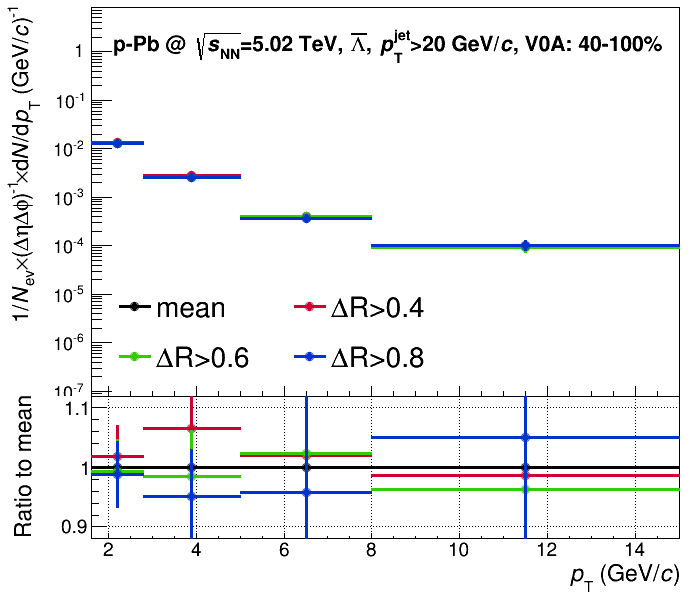
\includegraphics[width=.32\textwidth]{c05Results/cAntiLa_Comp_OC_JE_V0A_040_100_PtJ20}
\caption{Normalized ${\rm OC}~\Vzeros$ with different $\Delta R$
         in $\pT^{\rm jet}>20~\GeVc$.}
\label{fig:c05RestulsCompOCPtJ20}
\end{center}
\end{figure}

The method used for the  feeddown subtraction for the inclusive $\Vzeros$
is introduced in~\cite{Ali2012:ana501}.
According to this method, the subtraction has to be applied before the
efficiency correction.

To apply the feeddown subtraction of the $\Vzeros$ in jets,
the following issues has to be considered:
\begin{itemize}
\item we have not measured the $\Xi$ produce inside jets yet;
\item the $\Vzeros$ produced inside jets are obtained by subtract the
      UE $\Vzeros$ from the JC $\Vzeros$ and the JC $\Vzeros$ are composed
      by the following four components:
      \begin{equation}\label{eq:c05CompsInJC}
      {\rm JC}={\rm JC}_{\rm H}+
               {\rm JC}_{\rm F}+{\rm UE}_{\rm H}+{\rm UE}_{\rm F},
      \end{equation}
      where,
      \begin{itemize}
      \item ${\rm JC}_{\rm H}~\Vzeros$
            is the primary $\Vzeros$ produced inside jets and
            they are what we are going to measured in this analysis;
      \item ${\rm JC}_{\rm F}~\Vzeros$
            is the feeddown $\Vzeros$ matched with the jets;
      \item ${\rm UE}_{\rm H}~\Vzeros$
            is the primary $\Vzeros$ in matched with the jets but
            from the underlying event;
      \item ${\rm UE}_{\rm F}$ is the feeddown $\Vzeros$ matched with jets
            but from the underlying event.
      \end{itemize}
\end{itemize}

Since the efficiency correction will not change the ratios of
${\rm JC}_{\rm H}~\Vzeros/{\rm JC}_{\rm F}~\Vzeros$ and
${\rm UE}_{\rm H}~\Vzeros/{\rm UE}_{\rm F}~\Vzeros$
in the JC $\Vzero$ component.
the following steps are used to subtract the feeddown contributions
for the $\Vzero$ produced inside jets:
\begin{enumerate}
\item apply the efficiency correction for both JC and UE $\Vzeros$ without
      the feeddown subtraction;
\item subtract the normalized UE component from the JC $\Vzeros$,
      in this procedure,
      the last two terms in eq.~{\ref{eq:c05CompsInJC}} are subtracted;
\item subtract the feeddown $\Vzeros$ matched with
      jets (${\rm JC}_{\rm F}~\Vzeros$) according to the estimated
      fedddown fraction.
\end{enumerate}

The uncertainty of this feeddown subtraction strategy will be
discussed in section~\ref{sec:c06SystFd}.


\begin{table}[htdp]
\begin{center}
\begin{tabular}{ c c }
\hline
selection                           & value \\
\hline
track Kink index                    & $<1$ \\
$|\eta|$                            & $<0.8$ \\
TPC refit flag                      & kTRUE \\
number of crossed rows in TPC       & $>70$ \\
number of findable rows in TPC      & $>0$ \\
crossed rows / findable rows ratio  & $>0.8$ \\
TPC ${\rm d}E/{\rm d}x$             & $<5\sigma$ \\
\hline
\end{tabular}
\end{center}
\caption{Default selection cuts for $\Vzero$ daughter tracks.}
\label{tab:daughtercuts}
\end{table}

In data, the $\Vzero$ candidates are selected by several set of cuts:
\begin{itemize}
\item $\Vzero$ secondary vertex reconstruction with $\chi^{2}<33$;
\item topological selection;
\item daughter track selection;
\item proper lifetime ($mL/p$):
      default value for $\Kshort$ ($\Lambda$) is $<20$~cm ($<30$~cm);
\item invriant mass restriction (as a function of $\Vzero$ $\pT$):
      \begin{itemize}
      \item $\Kshort$:
            \begin{itemize}
            \item upper band: $0.563707+0.0114979\times\pT$,
            \item lower band: $0.430006-0.0110029\times\pT$,
            \end{itemize}
      \item $\Lambda$ and $\AntiLa$:
            \begin{itemize}
            \item upper band:
                  $1.13688+0.00527838\pT+0.084222\times\exp(-3.80595\pT)$,
            \item lower band:
                  $1.09501-0.00523272\pT-0.075269\times\exp(-3.46339\pT)$;
            \end{itemize}
      \end{itemize}
\item competing $\Vzero$ rejection:
      \begin{itemize}
      \item $\Kshort$: $|M_{{\rm p}\pim}-M_{\Lambda}|>0.005~\gevcc$ and 
                       $|M_{\pbar\pip}-M_{\AntiLa}|>0.005~\gevcc$,
      \item $\Lambda$ and $\AntiLa$: $|M_{\pip\pim}-M_{\Kshort}|>0.01~\gevcc$.
      \end{itemize}
\end{itemize}

In MC, the reconstructed $\Vzeros$ and the decay daughter tracks are identified with the information provided by the generator.

To implement the efficiency correction to the JC and OC $\Vzeros$ one has to
consider that,
the efficiency of $\Vzeros$ inside and outside jet cone could be different.
As a testing, we used to the following steps to check the efficiency of
JC $\Vzeros$
in the simulations:
\begin{enumerate}
\item reconstruct and select the jets in the simulations at
      detector level (with the reconstructed tracks) with the same criteria
      as in data,
\item match the physical primary $\Vzeros$ at particle level (the generated
      particles) to the reconstructed jets to build the denominator of
      the efficiency;
\item reproduce the steps in section~\ref{sec:c05V0JetMat} to obtain the
      number of JC $\Vzeros$ at detector level and use it to build the
      numerator of the efficiency.
\end{enumerate}
This procedure is summarized
in~\cite{Zimmermann:AliPWGJE20140401}~\footnote{There are two strategies for
the efficiency estimation of JC $\Vzeros$  in MC are proposed
in~\cite{Zimmermann:AliPWGJE20140401}.
The procedure introduced in this note is corresponding to the second one.}.

As discussed in section~\ref{sec:c03AnaStrategy},
to build the numerator of the $\Vzero$ efficiency,
the interpolated result from the fit in the side bands has to be subtracted
from the signal window.
Due to the bin counting ratio of the inclusive $\Vzeros$ in MC (as shown in
the right panel of figure~\ref{fig:c03CbinRatio}) is only $\sim 1\%$.
At here, the bin counting subtraction of the JC $\Vzeros$ in MC is done
by applying the bin counting ratio of the inclusive $\Vzeros$.
The uncertainty introduced by this procedure should have a order of $1\%$,
especially, in the low and intermedia $\pT$ regions.

\begin{figure}[htb]
\begin{center}
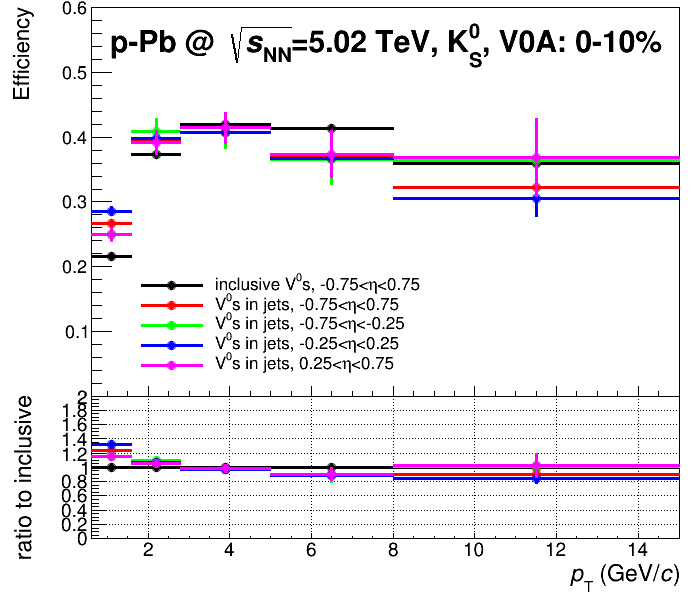
\includegraphics[width=.32\textwidth]{c05EffJetV0sMC/cKa_EffiJetEta_V0A_000_010}
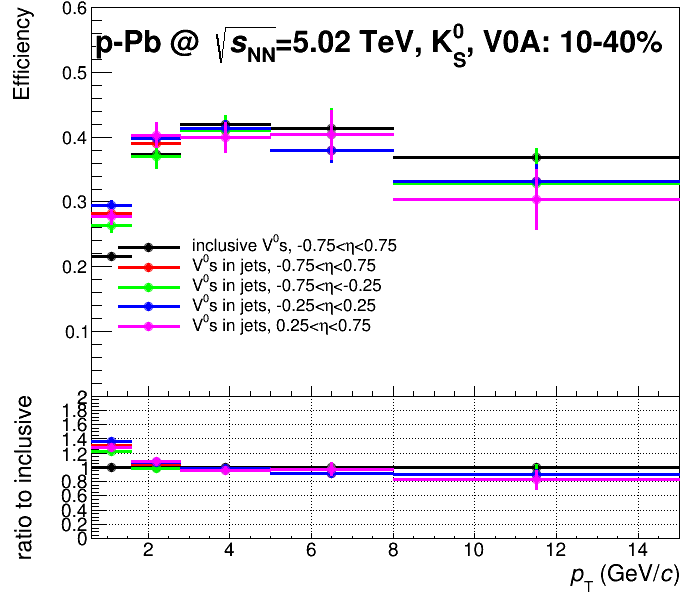
\includegraphics[width=.32\textwidth]{c05EffJetV0sMC/cKa_EffiJetEta_V0A_010_040}
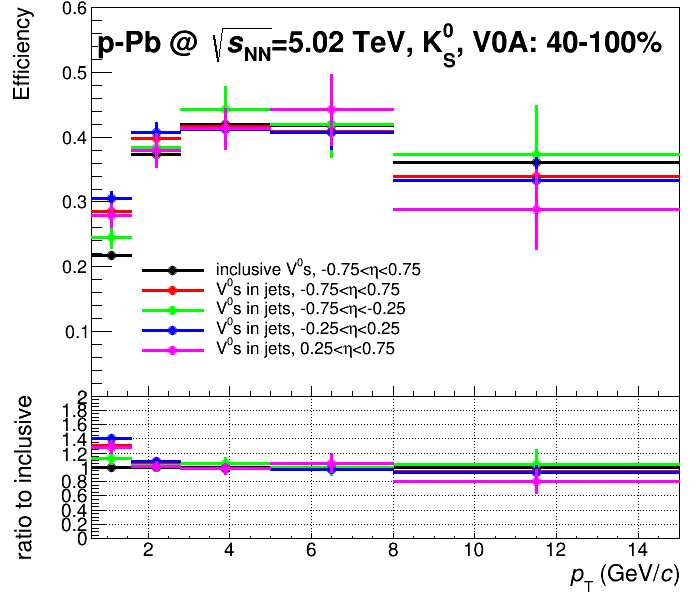
\includegraphics[width=.32\textwidth]{c05EffJetV0sMC/cKa_EffiJetEta_V0A_040_100}
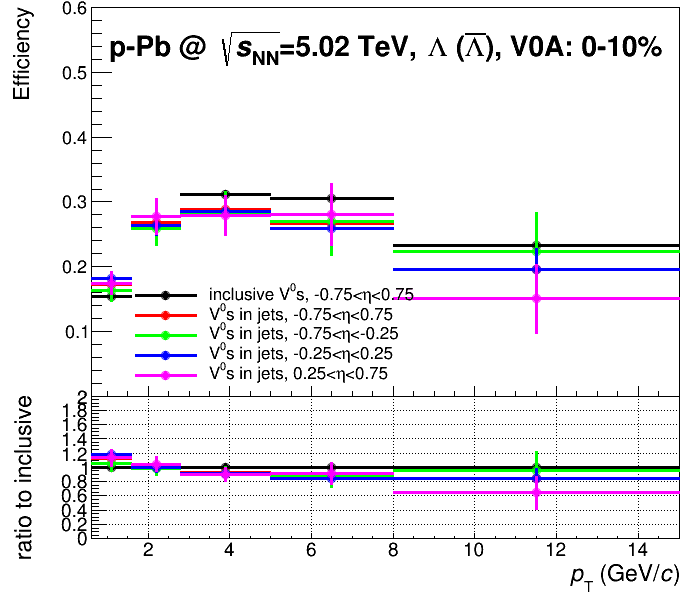
\includegraphics[width=.32\textwidth]{c05EffJetV0sMC/cLa_EffiJetEta_V0A_000_010}
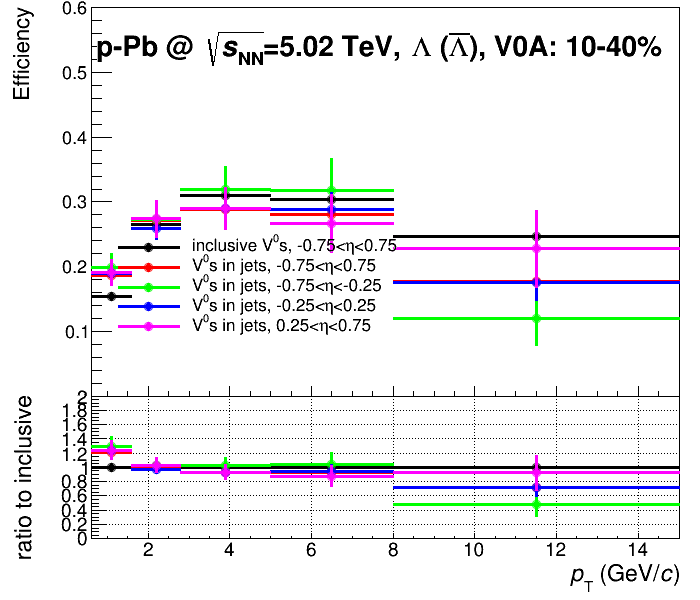
\includegraphics[width=.32\textwidth]{c05EffJetV0sMC/cLa_EffiJetEta_V0A_010_040}
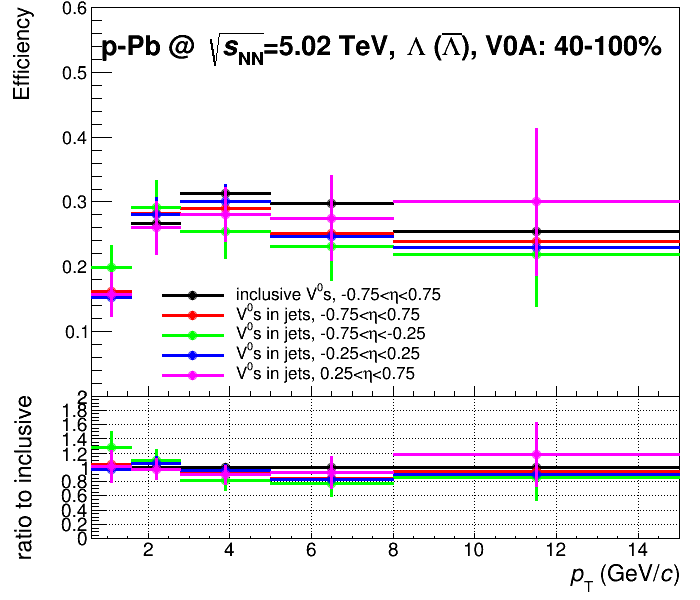
\includegraphics[width=.32\textwidth]{c05EffJetV0sMC/cLa_EffiJetEta_V0A_040_100}
\caption{Efficiency of $\Vzeros$ in jets as a function of $\pT$
         in three event multiplicity bins in simulations.
         The results are obtained in $\pT^{\rm jet}>10~\GeVc$.}
\label{fig:c05EffiJetV0sMC}
\end{center}
\end{figure}

Figure~\ref{fig:c05EffiJetV0sMC} shows the efficiency of $\Vzeros$ with jets
in $\pT>10~\GeVc$.
The results are compared with those of the inclusive $\Vzeros$ as well as
the those obtained in three sub-$\eta$ bins.
In general, the efficinecy of $\Vzeros$ in jets is $\sim 20\%$ higher than
that of inclusive $\Vzeros$ in low $\pT$ region.
At high $\pT$, the efficiency of $\Vzeros$ in jets is consistent with
the efficiency of inclusive $\Vzeros$.
To deeply handle the efficiency correction of the JC and OC $\Vzeros$,
one has to understand the reason for the increasing of the efficiency
JC $\Vzeros$ w.~r.~t. that of inclusive $\Vzeros$ in the low $\pT$ region.

\subsubsection{$\eta$ modified $\Vzero$ efficiency}
\label{sec:c05ScaledV0Effi}

\begin{figure}[htb]
\begin{center}
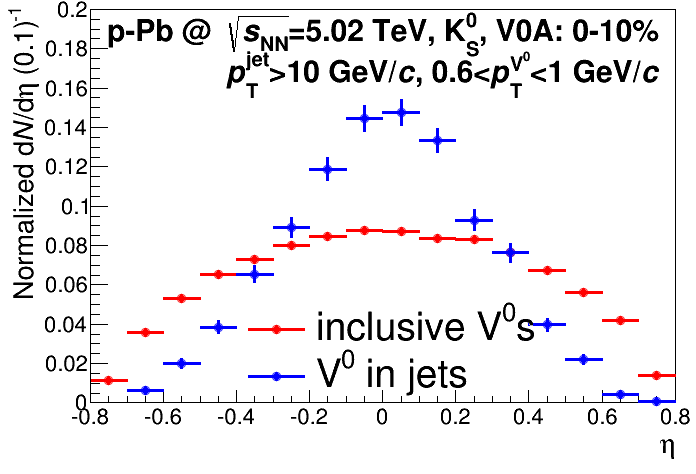
\includegraphics[width=.48\textwidth]{c05EffiV0Eta/cSpectra.png}
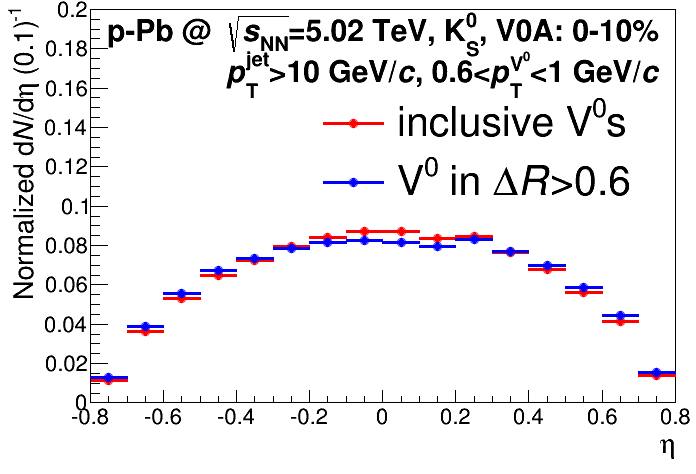
\includegraphics[width=.48\textwidth]{c05EffiV0Eta/cSpectra_OC}
\caption{Normalized $\eta$ distriubtion of $\Kshort$ in jets (left)
         and OC $\Kshort$ with $\Delta R>0.6$ (right) in data.
         The results are compared to the $\eta$ distriubtion of 
         inclusive and $\Kshort$.}
\label{fig:c05EffiJetV0Wgt}
\end{center}
\end{figure}

\begin{figure}[htb]
\begin{center}
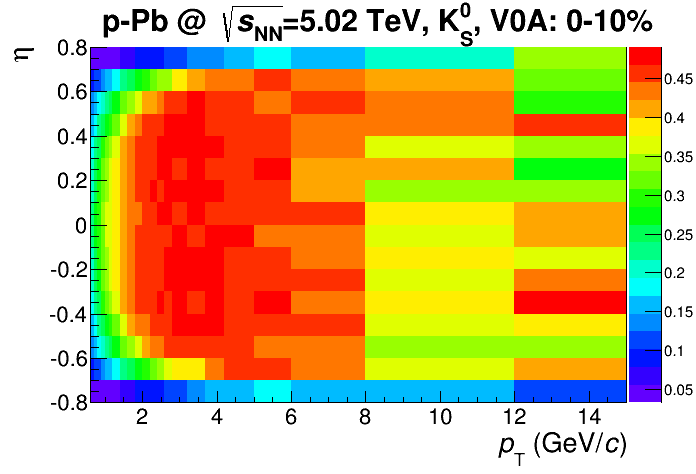
\includegraphics[width=.8\textwidth]{c05EffiV0Eta/cEfficiency_InclusiveV0}
\caption{2D efficiency of inclusive $\Vzeros$ as a function of $\pT$
         and $\eta$.}
\label{fig:c05EffiIncV02D}
\end{center}
\end{figure}

It has been shown that,
for the single $\Vzeros$, its efficiencies inside and outside the jets are
same~\cite{Kucera:AliPWGJE20140328}.
The difference between the efficiency of $\Vzeros$ in jets and
inclusive $\Vzeros$ is caused by the bias of the jet $\eta$ distribution.
Figure~\ref{fig:c05EffiJetV0Wgt} shows the normalized $\eta$ distribution
of JC $\Kshort$ candidates (left) and OC $\Kshort$ candidates
with $\Delta R_{\rm cut}>0.6$ (right) in $0.6<\pT<1~\GeVc$ in data.
The results are compared to the $\eta$ distribution of inclusive
and $\Kshort$ candidates.
The $\eta$ shape of JC $\Kshort$ candidates is modified by
the $\eta$ distribution of the jets.

As shown in figure~\ref{fig:c05EffiIncV02D},
the efficiency of inclusive $\Vzeros$ is non-uniform in $\eta$.
The integrated $\pT$-dependent $\Vzero$ efficiency can be treated as
weighted mean of the efficiency in the fine $\eta$ bins:
\begin{equation}\label{eq:c05WeightedEffi}
\varepsilon(\pT)=\frac{\sum_{\pT}r(\pT,\eta)}
                      {\sum_{\pT}g(\pT,\eta)}
 =\sum_{\pT}w(\pT,\eta)\varepsilon(\pT,\eta),
\end{equation}
where:
\begin{itemize}
\item $r(\pT,\eta)$ and $g(\pT,\eta)$ are the number of reconstructed and
      generated particles in each fine $\pT-\eta$ bin, respectively;
\item $w(\pT,\eta)=g(\pT,\eta)/\sum_{\pT}g(\pT,\eta)$ is the weight in the
      fine $\pT-\eta$ bins;
\item $\varepsilon(\pT,\eta)=r(\pT,\eta)/g(\pT,\eta)$ is the efficiency
      in the fine $\pT-\eta$ bins.
\end{itemize}
According to eq.~(\ref{eq:c05WeightedEffi}),
the bin has the larger counts will contribute the higher weight in the
integrated efficiency.
As show in the left panel of figure~\ref{fig:c05EffiJetV0Wgt},
the bin towards to $\eta=0$ in JC $\Vzero$ $\eta$ distribution has the
larger contribution in the integrated efficiency than that in the $\eta$
distribution of inclusive $\Vzeros$.
Due to the differential efficiency of $\Vzeros$ in the fine $\eta$ bin
towards to $\eta=0$ is higher than other,
it makes the increasing of the JC $\Vzero$ efficiency w.~r.~t. that of
the inclusive $\Vzeros$ in the low $\pT$
as shown in figure~\ref{fig:c05EffiJetV0sMC}.

To define the efficiency of the JC and OC $\Vzeros$ more precisely,
a scaling approach based on choosing a reference fine $\eta$ bin in data is
proposed~\cite{Zimmermann:AliPWGJE20140411}.
In this approach, the efficiency of JC and OC $\Vzeros$ in data is
calculated as:
\begin{equation}\label{eq:c05CorrEff}
\varepsilon_{\rm RD}(\pT)=
\frac{\sum_{\eta}n(\pT,\eta)}
     {\sum_{\eta}n(\pT,\eta)/\varepsilon_{\rm MC}(\pT,\eta)},
\end{equation}
where, $n(\pT,\eta)$ is the number of reconstructed $\Vzeros$ in the give
$\pT-\eta$ bin in data and $/\varepsilon_{\rm MC}(\pT,\eta)$ is the 2D
efficiency of inclusive $\Vzeros$ obtained in MC.
The basic consideration for this formula is according to the
efficiency of single $\Vzeros$ (either inside jets or outside jets) are the
same and it is described by the efficiency of the inclusive $\Vzeros$ in the
fine $\pT-\eta$ bins in MC.
The numerator are the reconstructed number of $\Vzeros$ in data,
while the denominator corresponds to the number of generated $\Vzeros$ in data.
In this case, the formula eq.~(\ref{eq:c05CorrEff}) can not only be used to
calculate the efficiency of the JC and OC $\Vzeros$ but also be used to
correct the efficiency of inclusive $\Vzeros$ as well as the efficiency
of NJ $\Vzeros$.

As discussed in section~\ref{sec:c03AnaStrategy} and
section~\ref{sec:c05V0EffiMC},
the interpolated bin counting fit results in data and MC have to be
subtracted in the term of $n(\pT,\eta)$ and the numerator
in the term of $\varepsilon_{\rm MC}(\pT,\eta)$ in eq.~(\ref{eq:c05CorrEff}),
respectively.
But due to the restriction of the statistics,
is it hard to make the stable bin counting fit in the side bands
in the fine $\pT-\eta$ bins in both data and MC.
In the implementation, we assume the bin counting ratio $R_{\rm Cbin}$,
which defined in eq.~(\ref{eq:c03CbinR}),
is independent on $\eta$ in both data and
MC (the uncertainty introduced by this assumption will
be discussed in section~\ref{sec:c06SystSingleV0s}).
And the efficiency calculation in this analysis is modified as:
\begin{equation}\label{eq:c05CorrEffImp}
\varepsilon_{\rm RD}(\pT)=
\frac{f_{\rm Cbin}^{\rm MC}(\pT)\cdot\sum_{\eta}n(\pT,\eta)}
     {\sum_{\eta}n(\pT,\eta)/\varepsilon_{\rm MC}(\pT,\eta)},
\end{equation}
where $f_{\rm Cbin}^{\rm MC}(\pT)=
       R_{\rm Cbin}^{\rm MC}(\pT)/(1+R_{\rm Cbin}^{\rm MC}(\pT))$,
$R_{\rm Cbin}^{\rm MC}(\pT)$ is the $\pT$-dependent bin counting ratio
in MC as show in the right panel of figure~\ref{fig:c03CbinRatio}.
Then in eq.~(\ref{eq:c05CorrEffImp}) the term of $n(\pT,\eta)$ and the
numerator in the term of $\varepsilon_{\rm MC}(\pT,\eta)$ now correspond to
the number of $\Vzero$ candidates (without the bin counting subtraction) in
each fine $\pT-\eta$ bin.

\begin{figure}[htb]
\begin{center}
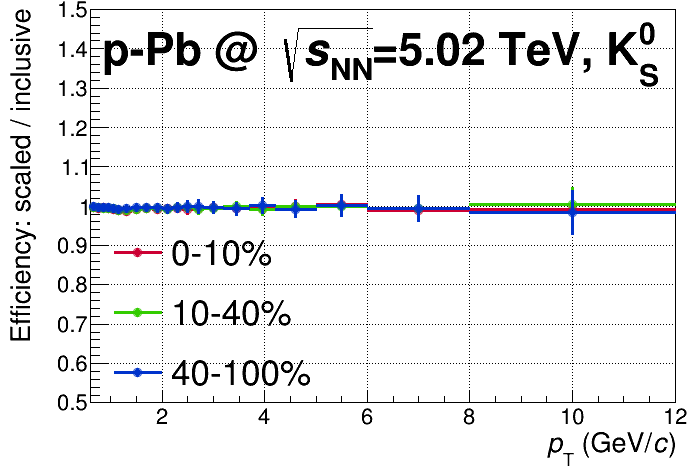
\includegraphics[width=.32\textwidth]{c05ScaledV0Effi/cCompEffIncl_Kshort}
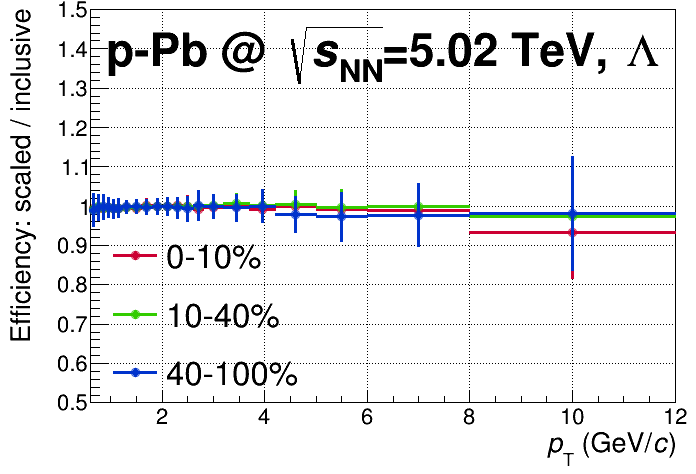
\includegraphics[width=.32\textwidth]{c05ScaledV0Effi/cCompEffIncl_Lambda}
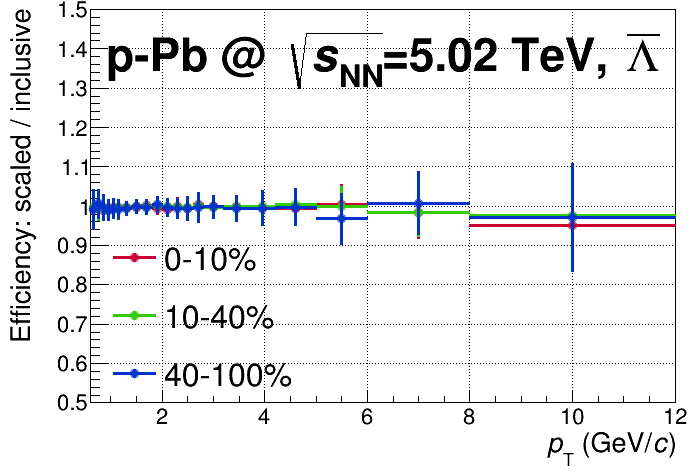
\includegraphics[width=.32\textwidth]{c05ScaledV0Effi/cCompEffIncl_AntiLa}
\caption{The ratio between the scaled inclusive $\Vzero$ efficiency
         calculated by using eq.~(\ref{eq:c05CorrEffImp}) and the
         inclusive $\Vzero$ efficiency in MC as shown
         in figure~\ref{fig:c05EffiIncV0s}.}
\label{fig:c05CompScaledEff}
\end{center}
\end{figure}

\begin{figure}[htb]
\begin{center}
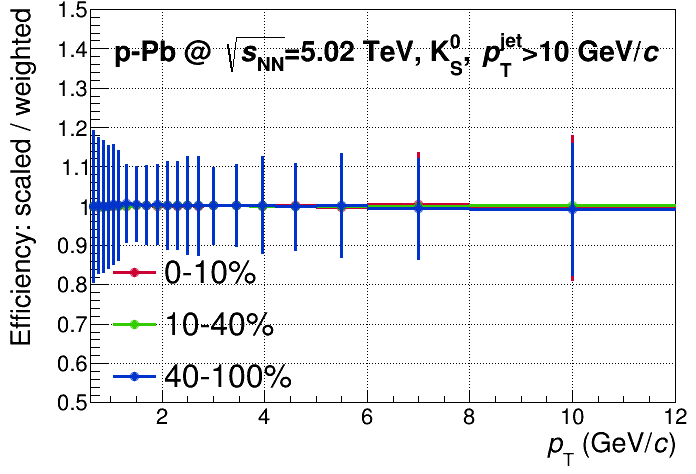
\includegraphics[width=.32\textwidth]{c05ScaledV0Effi/cCompEffWght_Kshort_PtJ10_JC}
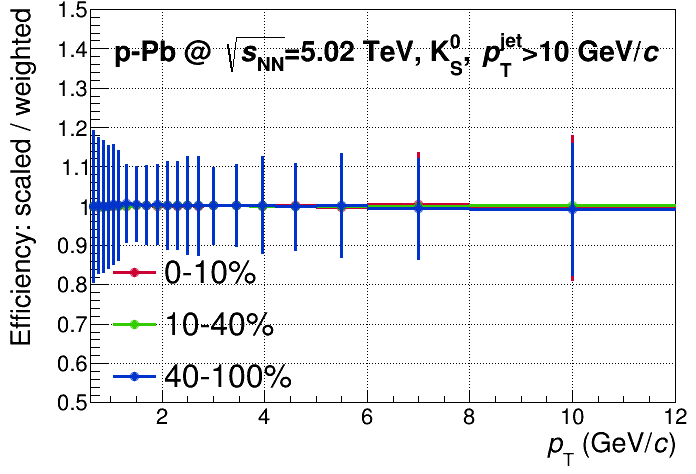
\includegraphics[width=.32\textwidth]{c05ScaledV0Effi/cCompEffWght_Kshort_PtJ10_JC}
\includegraphics[width=.32\textwidth]{c05ScaledV0Effi/cCompEffWght_Kshort_PtJ10_JC}
\caption{The ratio between the scaled JC $\Vzero$ efficiency calculated by
         using eq.~(\ref{eq:c05CorrEffImp}) and the JC $\Vzero$ efficiency
         calculated by the weighting approach described in
         appendix~\ref{sec:a01WghtV0Effi}.
         The results are obtained in $\pT^{\rm jet}>10~\GeVc$.}
\label{fig:c05CompScaledWghtPtJ10JC}
\end{center}
\end{figure}

\begin{figure}[htb]
\begin{center}
\includegraphics[width=.32\textwidth]{c05ScaledV0Effi/cCompEffWght_Kshort_PtJ10_OC06}
\includegraphics[width=.32\textwidth]{c05ScaledV0Effi/cCompEffWght_Kshort_PtJ10_OC06}
\includegraphics[width=.32\textwidth]{c05ScaledV0Effi/cCompEffWght_Kshort_PtJ10_OC06}
\caption{The ratio between the scaled OC $\Vzero$ efficiency calculated by
         using eq.~(\ref{eq:c05CorrEffImp}) and the OC $\Vzero$ efficiency
         calculated by the weighting approach described in
         appendix~\ref{sec:a01WghtV0Effi}.
         The results are obtained in $\pT^{\rm jet}>10~\GeVc$.
         The OC $\Vzeros$ are obtained with $\Delta R_{\rm cut}=0.6$.}
\label{fig:c05CompScaledWghtPtJ10OC06}
\end{center}
\end{figure}

\begin{figure}[htb]
\begin{center}
\includegraphics[width=.32\textwidth]{c05ScaledV0Effi/cCompEffWght_Kshort_PtJ05_NJ}
\includegraphics[width=.32\textwidth]{c05ScaledV0Effi/cCompEffWght_Kshort_PtJ05_NJ}
\includegraphics[width=.32\textwidth]{c05ScaledV0Effi/cCompEffWght_Kshort_PtJ05_NJ}
\caption{The ratio between the scaled NJ $\Vzero$ efficiency calculated by
         using eq.~(\ref{eq:c05CorrEffImp}) and the NJ $\Vzero$ efficiency
         calculated by the weighting approach described in
         appendix~\ref{sec:a01WghtV0Effi}.}
\label{fig:c05CompScaledWghtPtJ10NJ}
\end{center}
\end{figure}

Figure~\ref{fig:c05CompScaledEff} shows the ratio of the inclusive $\Vzero$
efficiency calculated by the scaling approach according
to eq.~(\ref{eq:c05CorrEffImp}) and the efficiency of
inclusive $\Vzeros$ in MC which is shown in figure~\ref{fig:c05EffiIncV0s}
in three event centrality bins.
In general, the discrepancy between the efficiency calculated by this
two approaches is $\sim 1\%$.
The ratio of the efficiency of the JC, OC and NJ $\Vzeros$ calculated by the
scaling approaching and those calculated by a weighting approach (introduced
in appendix~\ref{sec:a01WghtV0Effi}) are shown in
figure~\ref{fig:c05CompScaledWghtPtJ10JC},
figure~\ref{fig:c05CompScaledWghtPtJ10OC06} and
figure~\ref{fig:c05CompScaledWghtPtJ10NJ}, respectively.
The maximum deviation between the efficiencies obtained by these two methods
is $\sim 5\%$.

Please note that,
the error bars on the ratios in the figures are the statistic uncertainty
propagated by ROOT.
And indeed, the uncertainty propagation in the efficiency calculation is not
straight forward.
The details for the uncertainty will be discussed
in section~\ref{sec:c06StatErrors}.
%% data sample

These event estimators are discussed in detail in \cite{Adam:2014qja}. The data was analyzed in fractions of the total sample of 0-10\%, 10-40\%, 40-100\%.

The corresponding fractions of the data sample together with the mean charge-particle multiplicity densities ~($\avg{\dNdeta}$) within $| \hlab |<0.5$ in each V0A class are summarized in Tab.~\ref{tab:multclasses}.  
These are obtained using the method presented in~\cite{ALICE:2012xs} and are corrected for acceptance and
tracking efficiency as well as for contamination by secondary
particles. Contrary to our earlier measurement of $\avg{\dNdeta}$~\cite{ALICE:2012xs}, the values
in Tab.~\ref{tab:multclasses} are not corrected for trigger and
vertex-reconstruction efficiency, which is of the order of 2\% for NSD
events~\cite{ALICE:2012xs}. The same holds true for the \pt\
distributions, which are presented in the next section.

\begin{table}[t] 
  \centering
  \begin{tabular*}{\linewidth}{@{\extracolsep{\fill}}ccc}
    \hline
    &&\\[-0.7em]
     Event & V0A range & $\avg{\dNdeta}$\\
     class & \footnotesize{(arb. unit)} & \footnotesize{$|\hlab|<0.5$}\\[0.3em]
    \hline
    &&\\[-0.7em]
    0--10\%   & $>$ 187  & 40.6 $\pm$ 0.9 \\[0.3em]
    10--40\%  & 89-187   & 25.6 $\pm$ 0.6 \\[0.3em]
    40--100\% & $<$ 89   & 10.1 $\pm$ 0.2 \\[0.3em]
    \hline
  \end{tabular*}
  \caption{Definition of the event classes as fractions of the analyzed event sample and their corresponding $\avg{\dNdeta}$ within $|\hlab|<0.5$ (systematic uncertainties only, statistical uncertainties are negligible). \ask{Do we need this table? Also for ZNA?} }
  \label{tab:multclasses}
\end{table}

In contract to \PbPb collisions, the large multiplicity fluctuations in \pPb\ collisions, generate a dynamical bias in centrality classes based on particle multiplicity.
The results are also presented for tha ZNA estimator that suffers from signigicantly less biases~\cite{Adam:2014qja} providing, however, a smaller dynamic range of in the sensitivity to the event activity.

%% end data sample


There are two sets of MC simulations have been used in this analysis:
\begin{itemize}
\item DPMjet simulations: for the $\Vzero$ efficiency calculations
      and \lda\ and \alda\ feeddown correction;
\item PYTHIA simulations: used to build the detector response matrix for jets.
\end{itemize}
The details for each of the simulation sample are listed in the following.

\subsubsection{PYTHIA simulations}\label{sec:03PySampleMC}

\begin{itemize}
\item \pp\ collisions at \sqrtsnn{5.02};
\item data sample: LHC13b4 with LHC13b anchors;
\item a Lorentz boost has to be applied for the rapidity shift in p--Pb system;
\item events generated in 10 $\pT$-hard bins.
\end{itemize}


In addition, pA collisions allow for the
investigation of fundamental properties of QCD: the relevant part of
the initial state nuclear wave function extends to very low fractional
parton momentum $x$ and very high gluon densities, where parton
shadowing and novel phenomena like saturation, e.g. as implemented in
the Color Glass Condensate model (CGC), may become
apparent~\cite{McLerran:1993ni, Gelis:2010nm}. \ask{this is mentioned later when discussing jets}


\begin{table}[t] 
  \centering
  \begin{tabular*}{\linewidth}{@{\extracolsep{\fill}}ccc}
    \hline
    &&\\[-0.7em]
     Event & V0A range & $\avg{\dNdeta}$\\
     class & \footnotesize{(arb. unit)} & \footnotesize{$|\hlab|<0.5$}\\[0.3em]
    \hline
    &&\\[-0.7em]
    0--5\%    & $>$ 227  & 45   $\pm$ 1   \\[0.3em]
    5--10\%   & 187--227 & 36.2 $\pm$ 0.8 \\[0.3em]
    10--20\%  & 142--187 & 30.5 $\pm$ 0.7 \\[0.3em]
    20--40\%  & 89--142  & 23.2 $\pm$ 0.5 \\[0.3em] 
    40--60\%  & 52--89   & 16.1 $\pm$ 0.4 \\[0.3em]
    60--80\%  & 22--52   & 9.8  $\pm$ 0.2 \\[0.3em]
    80--100\% & $<$ 22   & 4.4  $\pm$ 0.1 \\[0.3em]
    \hline
  \end{tabular*}
  \caption{Definition of the event classes as fractions of the analyzed event sample and their corresponding $\avg{\dNdeta}$ within $|\hlab|<0.5$ (systematic uncertainties only, statistical uncertainties are negligible). }
  \label{tab:multclasses}
\end{table}


The relative standard deviation of the track multiplicity
distribution for the event classes defined in
Table~\ref{tab:multclasses} ranges from 78\% to 29\% for
the 80--100\% and 0--5\% classes, respectively. It should be noted
that the average multiplicity in the 80-100\% bin is well below the
corresponding multiplicity in pp minimum-bias
collisions~\cite{Aamodt:1260702} and therefore likely to be subject to
a strong selection bias. 

@article{ALICEdetector,
	Abstract = {ALICE (A Large Ion Collider Experiment) is a general-purpose, heavy-ion detector at the CERN LHC which focuses on QCD, the strong-interaction sector of the Standard Model. It is designed to address the physics of strongly interacting matter and the quark-gluon plasma at extreme values of energy density and temperature in nucleus-nucleus collisions. Besides running with Pb ions, the physics programme includes collisions with lighter ions, lower energy running and dedicated proton-nucleus runs. ALICE will also take data with proton beams at the top LHC energy to collect reference data for the heavy-ion programme and to address several QCD topics for which ALICE is complementary to the other LHC detectors. The ALICE detector has been built by a collaboration including currently over 1000 physicists and engineers from 105 Institutes in 30 countries. Its overall dimensions are 16 × 16 × 26 m 3 with a total weight of approximately 10 000 t. The experiment consists of 18 different detector systems each with its own specific technology choice and design constraints, driven both by the physics requirements and the experimental conditions expected at LHC. The most stringent design constraint is to cope with the extreme particle multiplicity anticipated in central Pb-Pb collisions. The different subsystems were optimized to provide high-momentum resolution as well as excellent Particle Identification (PID) over a broad range in momentum, up to the highest multiplicities predicted for LHC. This will allow for comprehensive studies of hadrons, electrons, muons, and photons produced in the collision of heavy nuclei. Most detector systems are scheduled to be installed and ready for data taking by mid-2008 when the LHC is scheduled to start operation, with the exception of parts of the Photon Spectrometer (PHOS), Transition Radiation Detector (TRD) and Electro Magnetic Calorimeter (EMCal). These detectors will be completed for the high-luminosity ion run expected in 2010. This paper describes in detail the detector components as installed for the first data taking in the summer of 2008.},
	Author = {K Aamodt et al.},
	Collaboration = {The ALICE Collaboration},
	Date-Added = {2014-08-06 15:34:42 +0000},
	Date-Modified = {2014-08-06 15:34:42 +0000},
	Journal = {Journal of Instrumentation},
	Number = {08},
	Pages = {S08002},
	Title = {The ALICE experiment at the CERN LHC},
	Url = {http://stacks.iop.org/1748-0221/3/i=08/a=S08002},
	Volume = {3},
	Year = {2008},
	Bdsk-Url-1 = {http://stacks.iop.org/1748-0221/3/i=08/a=S08002}}


@article{Alme2010316,
title = "The \{ALICE\} TPC, a large 3-dimensional tracking device with fast readout for ultra-high multiplicity events ",
journal = "Nuclear Instruments and Methods in Physics Research Section A: Accelerators, Spectrometers, Detectors and Associated Equipment ",
volume = "622",
number = "1",
pages = "316 - 367",
year = "2010",
note = "",
issn = "0168-9002",
doi = "http://dx.doi.org/10.1016/j.nima.2010.04.042",
url = "http://www.sciencedirect.com/science/article/pii/S0168900210008910",
author = "J. Alme and Y. Andres and H. Appelshäuser and S. Bablok and N. Bialas and R. Bolgen and U. Bonnes and R. Bramm and P. Braun-Munzinger and R. Campagnolo and P. Christiansen and A. Dobrin and C. Engster and D. Fehlker and Y. Foka and U. Frankenfeld and J.J. Gaardhøje and C. Garabatos and P. Glässel and C. Gonzalez Gutierrez and P. Gros and H.-A. Gustafsson and H. Helstrup and M. Hoch and M. Ivanov and R. Janik and A. Junique and A. Kalweit and R. Keidel and S. Kniege and M. Kowalski and D.T. Larsen and Y. Lesenechal and P. Lenoir and N. Lindegaard and C. Lippmann and M. Mager and M. Mast and A. Matyja and M. Munkejord and L. Musa and B.S. Nielsen and V. Nikolic and H. Oeschler and E.K. Olsen and A. Oskarsson and L. Osterman and M. Pikna and A. Rehman and G. Renault and R. Renfordt and S. Rossegger and D. Röhrich and K. Røed and M. Richter and G. Rueshmann and A. Rybicki and H. Sann and H.-R. Schmidt and M. Siska and B. Sitár and C. Soegaard and H.-K. Soltveit and D. Soyk and J. Stachel and H. Stelzer and E. Stenlund and R. Stock and P. Strmeň and I. Szarka and K. Ullaland and D. Vranic and R. Veenhof and J. Westergaard and J. Wiechula and B. Windelband",
keywords = "\{ALICE\}",
keywords = "Time Projection Chamber "
}

@article{Alme2010316,
title = "The \{ALICE\} TPC, a large 3-dimensional tracking device with fast readout for ultra-high multiplicity events ",
journal = "Nuclear Instruments and Methods in Physics Research Section A: Accelerators, Spectrometers, Detectors and Associated Equipment ",
volume = "622",
number = "1",
pages = "316 - 367",
year = "2010",
note = "",
issn = "0168-9002",
doi = "http://dx.doi.org/10.1016/j.nima.2010.04.042",
url = "http://www.sciencedirect.com/science/article/pii/S0168900210008910",
author = "Alme, J. and others",
Collaboration = {ALICE Collaboration},
keywords = "\{ALICE\}",
keywords = "Time Projection Chamber "
}

\ask{The jet part - needs adjustments as well - from the pPb RAA.}

Jets are the observable final state of a fragmenting parton produced e.g. in scattering of partons in nuclei with a large momentum  transfer, $Q^2$.  
%
At sufficiently large $Q^2$, the jet production cross section is
computable since it can be factorized into the non-perturbative parton distribution
and fragmentation functions and the  cross section of partonic scatterings, which is calculable
in perturbative QCD (pQCD) \cite{Col85a}.
%
Jet measurements in $\pPb$ and their comparison to $\pp$ provide a tool to better
constrain effects of (cold) nuclear matter on these factors. 
%
In particular, they can be used to examine the role of a modification of the initial distribution
of quarks and gluons, e.g. shadowing effects and gluon
saturation \cite{McLerran:2001sr,Salgado:2011wc}, and the impact of
multiple scatterings and hadronic re-interactions in the initial and
final state \cite{Krzywicki:1979gv,Accardi:2007in}.

In central heavy-ion collisions, the production of jets and high-$\pt$
particles is strongly modified: in $\PbPb$ collisions at the LHC, the
observed hadron yields are suppressed  by up to a factor of seven  compared
to $\pp$ collisions, approaching a factor of two suppression at high $\pt$
\cite{Aamodt:2010jd,Aamodt:2011vg,CMS:2012aa}.
% 
A similar suppression is also observed for reconstructed jets in
central $\PbPb$ \cite{Aad:2010bu,Chatrchyan:2012nia,Aad:2012vca,Abelev:2013kqa,Aad:2014bxa}.
%
This phenomenon, referred to as \emph{jet quenching}, has also been
observed previously in high-$\pt$ particle production in central
$\AuAu$ collisions at RHIC
\cite{Adcox:2001jp,Adler:2003qi,Ada03b,Adams:2003im,Arsene:2003yk,Back:2003qr}.
%
It is attributed to the creation of a quark-gluon plasma (QGP) in the
final state, where hard scattered partons radiate gluons in strong
interactions  with the medium, resulting  in  an energy loss of the
leading parton and a modified fragmentation pattern as predicted in \cite{Gyulassy:1990ye,Baier:1994bd}.
%

Initially, $\pPb$ collisions have been seen as the testing ground for
isolated cold nuclear matter effects, without the formation of a hot and dense medium.
% 
However, recent results on low-$\pt$ particle production and long
range correlations in $\pPb$ collisions at \sqrtsnn{5.02} \cite{CMS:2012qk,Abelev:2012ola,Aad:2013fja,Abelev:2013wsa} exhibit features of collective behavior, similar to those
found in $\PbPb$ collisions, where they are attributed to the creation of a QGP. 
%
At high $\pt$, results on the production of unidentified charged
particles
\cite{ALICE:2012mj,Abelev:2014dsa,Khachatryan:2015xaa,ATLAS-CONF-2014-029}
and jets \cite{ATLAS:2014cpa,Chatrchyan:2014hqa} in $\pPb$ collisions at \sqrtsnn{5.02} are
consistent with the absence of a strong final state suppression. 
%
The measurement of jets in $\pPb$ collisions compared to single hadrons tests the parton fragmentation beyond the leading particle with the inclusion of low-$\pt$ and large-angle fragments.

A jet is defined experimentally by the algorithm that combines the measured detector information such as tracks and/or calorimeter cells into jet objects and by the parameters of the algorithm. 
%
The desired properties of such algorithms in $\pp(\bar{\mathrm{p}})$ collisions and in the corresponding theoretical framework have been discussed e.g. in \cite{Huth:1990mi}. 
%
In general, jet algorithms aim to reconstruct the kinematic properties of the initial parton with as little dependence on the details of its fragmentation process as possible, i.e. the algorithms should yield consistent results when applied in a theoretical calculation at any stage of a parton shower and at final state particle level.
%
A particularly well suited class of algorithms in this context are those using sequential recombination schemes, which are infrared and collinear safe, in contrast to many conceptually simpler cone algorithms.
%
The computationally optimized implementation of
sequential recombination algorithms in the FastJet package
\cite{Cacciari:2005hq} facilitates their applicability also in collision systems with high multiplicity and thereby the comparison of results obtained with the same jet
algorithms in $\pp$, $\pPb$, and $\PbPb$ collisions.
%
An additional complication in the context of jet reconstruction in high-multiplicity events arises from the large background particle density, i.e. particles in the same aperture as the jet that are not related to the initial hard scattering. 
%
This background can be subtracted on an event-by-event basis 
and the impact on the reconstructed jet observable needs to be evaluated carefully \cite{Cacciari:2011tm,Abelev:2013kqa,Abelev:2012ej}. 

%

%% this is temperature, particle ratios, Et measurement from CMS
To characterize the physical properties of the short lived QGP (lifetime of about
10 fm/c \cite{Aamodt:2010jj}) the experimental studies use the auto-generated probes, such as
highly virtual partons created early in the collision, thermally
emitted photons, and particle correlations sensitive to the collective
expansion and the dynamics of the system.


The observed ratios of particle
abundances can be described in terms of statistical
models~\cite{Andronic:2008gu,Cleymans:2006xj}, which are governed
mainly by two parameters, the chemical freeze-out temperature \Tch\
and the baryochemical potential \muB\, which describes the net baryon
content of the system.
These models provide an accurate description of the data over a large
range of center-of-mass energies~(see
e.g.~\cite{BraunMunzinger:2003zz}), but a surprisingly large deviation
(about 50\%) was found for the proton production yield at the LHC~\cite{prl-spectra,
  Abelev:2013vea}.

Both a CGC
description~\cite{Dusling:2013oia}, based on initial state nonlinear
gluon interactions, as well as a model based on hydrodynamic
flow~\cite{Bozek:2012gr,Qin:2013bha}, assuming strong interactions
between final state partons or hadrons, can give a satisfactory
description of the \pPb\ correlation data. However, the modeling of
small systems such as \pPb\ is complicated because uncertainties
related to initial state geometrical fluctuations play a large role
and because viscous corrections may be too large for hydrodynamics to
be a reliable framework~\cite{Bzdak:2013zma}.


Therefore the assumption that final state dense matter effects can be
neglected in pA may no longer be valid.  


\subsection{Track selection}

The charged particles are reconstructed as tracks in ALICE central-barrel tracking detectors. They full cover the azimuth within $|\eta|<0.9$ and located inside a solenoidal magnet providing a $0.5$~T magnetic field.
The main detector components used for the reconstruction of charged particle
jets and $\Vzeros$ are Inner Tracking System (ITS) and
Time Projection Chamber (TPC).
The ITS is the innermost barrel detector,
it contains six cylindrical silicon layers grouped in three
individual systems (from the innermost to outwards):
the Silicon Pixel Detector (SPD),
the Silicon Drift Detector (SDD) and
the Silicon Strip Detector (SSD).
The TPC, follows outwards, is a cylindrical drift detector.
It is the main central barrel tracking device and provides
particle identification based on the track mean energy loss, \dedx, 
in the fill gas by measuring up to $159$ samples per track.

Several criteria are defined for track selection to ensure the track quality.
Each track is required to have been reconstructed in TPC with a minimum
number of TPC cluster and then successfully refitted in the final back propagation
to the primary vertex in detail in~\cite{Alessandro:2006yt}.

The tracks used for the charged jets reconstruction,
as described in~\cite{Abelev:2013kqa},
are required to have at least one hits in SPD with a cut on
the difference between the parameters of the track fit using
all the space points in ITS and TPC and, using only TPC clusters 
with the primary vertex position.
Due to the inefficiency region in SPD,
the azimuthal distribution of the selected tracks is not completely uniform.
To improve the azimuthal uniformity,
the tracks without hit in SPD are used for compensating.
For those tracks, to guarantee good momentum resolution,
the primary vertex is used as an additional constraint in the track fit.
This approach yields a very uniform tracking efficiency within
the acceptance and overcomes geometrical bias of the jet reconstruction
algorithm caused by the non-uniform acceptance effect.

For the $\Kshort$ and $\Lambda$ (the $\Vzeros$),
they are identified exploiting their weak decay topology in the channels
\begin{equation}
\begin{split}
\Kshort & \to  \pip\pim, \\
\Lambda (\AntiLa) & \to {\rm p}\pim (\pbar\pip),
\end{split}
\end{equation}
which have branching ratios of $69.2\%$ and $63.9\%$,
respectively~\cite{Beringer:1900zz}.
Depending on the lifetime,
they may cross several layers of the ITS before weakly decaying.
Therefore, no specific condition on the number of ITS hits is required for
the daughter tracks used for the $\Vzero$ candidates reconstruction.
There are other quality criteria are applied for selecting the daughter tracks of
weakly decaying particles which are not came from the primary vertex,
in detail in~\cite{Aamodt:2011zza}.
Since the tracks used for the jet reconstruction are constrained to the
primary vertex, \ask{is it correct?} most of them are primary particles.
They have a negligible overlap fraction
\ask{from Vit, to be checked}($<1\%$)
with the daughter tracks of $\Vzero$ candidates.
The reconstructions of jets and $\Vzeros$ are almost independent.
%%%%%%%%%%%%%%%%%%%%%%%%%%%%%%%%%%%%%%%%%%%%%%%%%%%%%%%%%%%%%%%%%%%%%%%%%%%%%%%


%%In the following, the studies of angular distributions of the \Vzero\ particles within jets are presented.
%The right panel of Fig.\ref{fig:L2Kratio} shows the \lda-to-\ks\ ratio for jets with $\pt>10\gevc$ but for particles that satisfy two conditions of the distance from the jet axis $R(\Vzero,\mathrm{jet}) < 0.2$ (shown in the left panel) and $R(\Vzero,\mathrm{jet}) < 0.4$. 
%For particles with $2<\pt<4\gevc$ the ratio for $R(\Vzero,\mathrm{jet}) < 0.4$ is enhanced by about 15\% over the narrower selection.
%in were obtained by simply dividing the corresponding densities. Figure \ref{fig:L2Kratio} shows the ratio... (left panel) and the ratio (right panel). 
%The L/K ratio for jets with \pt>20\gevc show a similar behavior (not shown).

\begin{figure}[htbp]
   \centering
   \includegraphics[width=0.47\textwidth]{cL2K_Pt_Mean_PtJE}
   \includegraphics[width=0.47\textwidth]{cL2K_Pt_Mean_PtJ10}  
   \caption{Ratio of \lda\ and \ks\ yields for three selections  }
   \label{fig:L2Kratio}
\end{figure}

To study closer the \pt\ evolution of particle distributions within the jets the raw \Vzero\ densities (no UE subtraction) are plotted as a function of the particle distance to the jet axis... \ref{fig:LKR}.

\begin{figure}[htbp]
   \centering
   \includegraphics[width=0.47\textwidth]{cKshort_VJ_Comp_PtJ10_PtV0_2d2_3d7}
   \includegraphics[width=0.47\textwidth]{cLambda_VJ_Comp_PtV0_2d2_3d7}
   \caption{caption}
   \label{fig:LKR}
\end{figure}

\begin{figure}[htbp]
   \centering
   \includegraphics[width=0.47\textwidth]{cRatioV_VJ_Mean_PtJ10}
   \caption{caption}
   \label{fig:L2KvsR}
\end{figure}


%%%%%% LateXit cuts

\newcommand{\pt}           {\ensuremath{p_{\mathrm{T}}}}
\newcommand{\Vzero}        {\ensuremath{{\rm V}^{0}}}
\frac{{\mathrm d}\rho^{\Vzero}}{{\mathrm d}\pt}={\mathrm d}\left(\frac{N^{\Vzero}}{A^{\Vzero}}\right)/{\mathrm d}\pt
\newline
{\mathrm d}\rho^{\Vzero}/{\mathrm d}\pt
\newline
\rho^{\Vzero}(\pt)=N^{\Vzero}/A^{\Vzero}(\pt)
\newline
{\ensuremath{ \rho^{\Vzero}(\pt) = N^{\Vzero} / A^{\Vzero} (\pt) }}

%% from the results section
To study closer the \pt\ evolution of the ratio associate with jets the ratios pf the raw \Vzero\ densities (no UE subtraction) were reconstructed as a function of the particle distance to the jet axis \ref{fig:LKR}.


